% \begin{dang}{LẬP PHƯƠNG TRÌNH TỔNG QUÁT MẶT PHẲNG}
% Để lập phương trình tổng quát của mặt phẳng $\left(\alpha\right)$ thông thường ta có 3 trường hợp cơ bản sau:\\
% $\textbf{Trường hợp 1:}$ Khi bài toán cho biết mặt phẳng $\left(\alpha\right)$ đi qua điểm $M_0 \left(x_0;y_0;z_0\right)$ và có một vectơ pháp tuyến $\overrightarrow{n} = \left(A;B;C\right)$ hoặc có hai vectơ chỉ phương $\overrightarrow{a}$, $\overrightarrow{b}$ (với $\overrightarrow{n} = \left[\overrightarrow{a},\overrightarrow{b}\right]$) thì viết dưới dạng sau:
% $$\left(\alpha\right) \colon A\left(x-x_0\right)+B\left(y-y_0\right)+C\left(z-z_0\right)=0$$
% $\textbf{Trường hợp 2:}$ Khi bài toán cho biết mặt phẳng $\left(\alpha\right)$ có một vectơ pháp tuyến $\overrightarrow{n} = \left(A;B;C\right)$ hoặc có hai vectơ chỉ phương $\overrightarrow{a}$, $\overrightarrow{b}$ (với $\overrightarrow{n} = \left[\overrightarrow{a},\overrightarrow{b}\right]$) và không tìm được điểm $M_0 \left(x_0;y_0;z_0\right) \in \left(\alpha\right)$ thì ta thực hiện các bước sau:
% \begin{itemize}
% 	\item $\textbf{Bước 1:}$ Viết phương trình mặt phẳng $\left(\alpha\right)$ dưới dạng:
% 	$$Ax+By+Cz+D=0$$
% 	\item $\textbf{Bước 2:}$ Sau đó dựa vào giả thiết bài toán để tìm giá trị $D$.
% \end{itemize}
% \begin{note}
% 	Dạng này, giả thiết có liên quan đến khoảng cách và góc liên quan đến mặt phẳng.
% \end{note}
% $\textbf{Trường hợp 3:}$ Khi bài toán cho biết mặt phẳng $\left(\alpha\right)$ đi qua điểm $M_0 \left(x_0;y_0;z_0\right)$ và giả thiết bài toán không cho vectơ pháp tuyến $\overrightarrow{n}$ hoặc không cho hai vectơ chỉ phương $\overrightarrow{a}$, $\overrightarrow{b}$ thì ta thực hiện các bước sau:
% \begin{itemize}
% 	\item $\textbf{Bước 1:}$ Gọi vectơ pháp tuyến của mặt phẳng $\left(\alpha\right)$ là $\overrightarrow{n} = \left(A;B;C\right)$ với $A^2+B^2+C^2 \neq 0$
% 	\item $\textbf{Bước 2:}$ Viết phương trình mặt phẳng $\left(\alpha\right)$ dưới dạng:
% 	$$\left(\alpha\right) \colon A\left(x-x_0\right)+B\left(y-y_0\right)+C\left(z-z_0\right)=0$$
% 	\item $\textbf{Bước 3:}$ Sau đó dựa vào giả thiết bài toán để tìm hai phương trình chứa $3$ ẩn $A$, $B$, $C$.
% 	\begin{note}
% 		\begin{itemize}
% 			\item Dạng này, giả thiết có liên quan đến khoảng cách và góc liên quan đến mặt phẳng
% 			\item Để giải tìm vectơ pháp tuyến của mặt phẳng đơn giản hơn thì gọi vectơ pháp tuyến của mặt phẳng là $\overrightarrow{n} = \left(1;B;C\right)$.
% 		\end{itemize}
% 	\end{note}
% \end{itemize}

\begin{dang}{Viết PTTQ MP khi biết điểm đi qua và một VTPT hoặc hai VTCP}
	\textbf{1. Lập phương trình tổng quát} của mặt phẳng đi qua điểm $M_0 \left(x_0;y_0;z_0\right)$ và biết một vectơ pháp tuyến $\overrightarrow{n} = \left(A;B;C\right)$\\
	Trong KG $Oxyz$, phương trình tổng quát của mặt phẳng đi qua điểm $M_0 \left(x_0;y_0;z_0\right)$ và có vectơ pháp tuyến $\overrightarrow{n}= \left(A;B;C\right)$ là:\\
	$$A\left(x-x_0\right) + B\left(y-y_0\right)+C\left(z-z_0\right) = 0$$
	hay $Ax+By+Cz+D=0$ với $D= -Ax_0-By_0-Cz_0$
	\begin{center}
		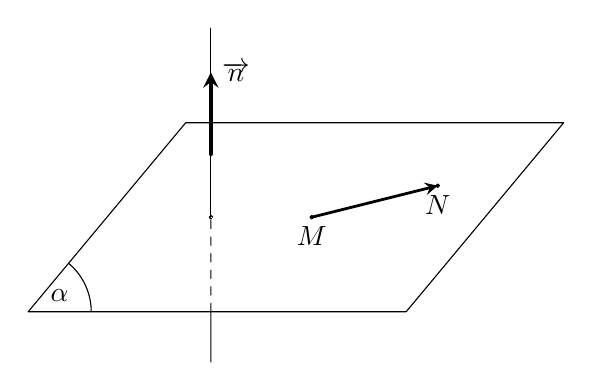
\begin{tikzpicture}[>=stealth,line join=round, line cap=round, scale=0.8]
			\coordinate (A) at (1.5,3);
			\coordinate (B) at (-1,0);
			\coordinate (C) at (5,0);
			\coordinate (D) at (7.5,3);
			\coordinate (I) at (1.9,1.5); \coordinate (J) at (1.9,4.5); \coordinate (K) at (1.9,-0.8);
			\coordinate (M) at (3.5,1.5);
			\coordinate (N) at (5.5,2);
			\begin{scope}
				\clip (A)--(B)--(C);
				\draw (B) circle (1);
			\end{scope}
			\draw (A)--(B)--(C)--(D)--(A);
			\draw (-0.8,0) node[above right]{$\alpha$};
			\draw (K)--(1.9,0); \draw [dashed] (1.9,0)--(I) circle (.8pt);  \draw (I)--(J);
			\draw (M) node[below]{$M$} circle (.8pt)--(N) node[below]{$N$} circle (.8pt);
			\draw[->,line width=1] (M)--(N);
			\draw[->,line width=1.4] (1.9,2.5)--(1.9,3.8) node[right]{$\overrightarrow{n}$};
		\end{tikzpicture}
	\end{center}
	$\textbf{Chú ý:}$
	\begin{enumerate}[a.]
		\item Mặt phẳng $\left(\alpha\right)$ có cặp vectơ chỉ phương $\overrightarrow{a}$, $\overrightarrow{b}$ ($\overrightarrow{a}$, $\overrightarrow{b}$ không cùng phương) thì mặt phẳng $\left(\alpha\right)$ có vectơ pháp tuyến $\overrightarrow{n}= \left[\overrightarrow{a},\overrightarrow{b}\right]$.
		\item Mặt phẳng $\left(\alpha\right)$ đi qua ba điểm $A$, $B$, $C$ không thẳng hàng thì có cặp vectơ chỉ phương $\overrightarrow{AB}$, $\overrightarrow{AC}$ nên mặt phẳng $\left(\alpha\right)$ có vectơ pháp tuyến $\overrightarrow{n} = \left[\overrightarrow{AB}, \overrightarrow{AC}\right]$.
		\item Dựa vào tính chất vuông góc, song song giữa mặt phẳng với mặt phẳng, giữa đường thẳng với mặt phẳng trong không gian để tìm vectơ chỉ phương, vectơ pháp tuyến của mặt phẳng cần lập.
		\begin{itemize}
			\item Hai mặt phẳng song song thì có cùng vectơ pháp tuyến.
			\item Hai mặt phẳng vuông góc thì vectơ chỉ phương của mặt phẳng này là vectơ pháp tuyến của mặt phẳng kia.
			\item Đường thẳng song song mặt phẳng thì vectơ chỉ phương của đường thẳng là vectơ chỉ phương của mặt phẳng.
			\item Đường thẳng vuông góc mặt phẳng thì vectơ chỉ phương của đường thẳng là vectơ pháp tuyến của mặt phẳng.
		\end{itemize}
	\end{enumerate}
	\textbf{2. Các trường hợp đặc biệt của mặt phẳng}
	\begin{enumerate}[a.]
		\item Phương trình mặt phẳng theo đoạn chắn\\
		Mặt phẳng $\left(\alpha\right)$ không đi qua gốc tọa độ $O$ và lần lượt cắt trục $Ox$ tại $A \left(a;0;0\right)$, cắt trục $Oy$ tại $B \left(0;b;0\right)$, cắt trục $Oz$ tại $C \left(0;0;c\right)$ có $\textbf{phương trình mặt phẳng theo đoạn chắn}$ là: $\dfrac{x}{a}+\dfrac{y}{b}+\dfrac{z}{c}=1$ với $a \cdot b \cdot c \neq 0$
		\begin{center}
			\begin{tikzpicture}[>=stealth,line join=round, line cap=round, scale=0.7]
				\coordinate (O) at (0,0); 
				\coordinate (A) at (-1.9,-1.9); \coordinate (C) at (0,3); \coordinate (B) at (3,0);
				\path[name path=trucy] (O)--(5,0);
				\path[name path=d1] (A)--(C);
				\path[name path=d2] (B)--(C);
				\path[name path=d3] (A)--(B);
				\path[name path=trucz] (O)--(0,5); \path[name path=trucx] (O)--(-4,-4);
				\path[name intersections={of=d1 and trucz, by=I}];  
				\path[name intersections={of=d1 and trucx, by=J}];
				\path[name intersections={of=d2 and trucy, by=K}]; 
				\draw [fill = blue!5] (I)--(J)--(K)--(I);
				\draw [->] (I)--(0,5) node[right]{$z$};\draw [->] (K)--(4,0) node[above right]{$y$}; \draw [->] (J)--(-3,-3) node[right]{$x$};
				\draw [dashed] (O) node[below]{$O$} circle (.8pt)--(I) node[left]{$C(0;0;c)$};
				\draw [dashed] (O)--(J) node[above left]{$A(a;0;0)$};
				\draw [dashed] (O)--(K) node[below right]{$B(0;b;0)$};
			\end{tikzpicture} 
		\end{center}
		\item Phương trình mặt phẳng đặc biệt\\
		Xét phương trình mặt phẳng $\left(\alpha\right) \colon Ax+By+Cz+D=0$ với $A^2+B^2+C^2 \neq 0$
		\begin{itemize}
			\item Nếu $D = 0$ thì mặt phẳng $\left(\alpha\right)$ đi qua gốc tọa độ $O$ và có dạng $\left(\alpha\right) \colon Ax+By+Cz=0$.
			\begin{center}
				\begin{tikzpicture}[>=stealth,line join=round, line cap=round, scale=0.8]
					%p1
					\coordinate (O) at (0,0); 
					\coordinate (x) at (-2,-2); 
					\coordinate (y) at (4,0); 
					\coordinate (z) at (0,3.5); 
					%p2
					\draw [->] (O) node[below]{$O$}--(x) node[below right]{$x$}; 
					\draw [->] (O)--(y) node[below]{$y$}; 
					\coordinate (A) at (3.3,2.5); \coordinate (B) at (-3,2);
					\draw [fill = blue!5] (A)--(O)--(B)--cycle;
					\path[name path=d1] (A)--(B);
					\path[name path=d2] (O)--(z);
					\path[name intersections={of=d1 and d2, by=M}];
					\draw [->] (M)--(z) node[right]{$z$}; \draw [dashed] (O)--(M);
					\draw (-2.5,2.1) node[below right]{$\left(\alpha\right)$};
					\draw (0.2,-2) node[right]{$Ax+By+Cz=0$};
				\end{tikzpicture}
			\end{center}
			\item Nếu $A=0$, $B \neq 0$, $C \neq 0$ thì mặt phẳng $\left(\alpha\right)$ song song hoặc chứa trục $Ox$.
			\item[+] Mặt phẳng $\left(\alpha\right)$ song song $Ox$ thì có dạng $\left(\alpha\right) \colon By+Cz+D=0$.(Hình 1)
			\item[+] Mặt phẳng $\left(\alpha\right)$ chứa trục $Ox$ thì có dạng $\left(\alpha\right) \colon By+Cz=0$.
			\item Nếu $A \neq 0$, $B = 0$, $C \neq 0$ thì mặt phẳng $\left(\alpha\right)$ song song hoặc chứa trục $Oy$.
			\item[+] Mặt phẳng $\left(\alpha\right)$ song song $Oy$ thì có dạng $\left(\alpha\right) \colon Ax+Cz+D=0$.(Hình 2)
			\item[+] Mặt phẳng $\left(\alpha\right)$ chứa trục $Oy$ thì có dạng $\left(\alpha\right) \colon Ax+Cz=0$.
			\item Nếu $A\neq 0$, $B \neq 0$, $C = 0$ thì mặt phẳng $\left(\alpha\right)$ song song hoặc chứa trục $Oz$.
			\item[+] Mặt phẳng $\left(\alpha\right)$ song song $Oz$ thì có dạng $\left(\alpha\right) \colon Ax+By+D=0$.(Hình 3)
			\item[+] Mặt phẳng $\left(\alpha\right)$ chứa trục $Oz$ thì có dạng $\left(\alpha\right) \colon Ax+By=0$.
			\item Nếu $A=B= 0$, $C \neq 0$ thì mặt phẳng $\left(\alpha\right)$ song song hoặc trùng với $\left(Oxy\right)$.
			\item[+] Mặt phẳng $\left(\alpha\right)$ song song $\left(Oxy\right)$ thì có dạng $\left(\alpha\right) \colon Cz+D=0$.(Hình 4)
			\item[+] Mặt phẳng $\left(\alpha\right)$ chứa $\left(Oxy\right)$ thì có dạng $\left(\alpha\right) \colon z=0$.
			\item Nếu $A=C= 0$, $B \neq 0$ thì mặt phẳng $\left(\alpha\right)$ song song hoặc trùng với $\left(Oxz\right)$.
			\item[+] Mặt phẳng $\left(\alpha\right)$ song song $\left(Oxz\right)$ thì có dạng $\left(\alpha\right) \colon By+D=0$.(Hình 5)
			\item[+] Mặt phẳng $\left(\alpha\right)$ chứa $\left(Oxz\right)$ thì có dạng $\left(\alpha\right) \colon y=0$.
			\item Nếu $B=C= 0$, $A \neq 0$ thì mặt phẳng $\left(\alpha\right)$ song song hoặc trùng với $\left(Oyz\right)$.
			\item[+] Mặt phẳng $\left(\alpha\right)$ song song $\left(Oyz\right)$ thì có dạng $\left(\alpha\right) \colon Ax+D=0$.(Hình 6)
			\item[+] Mặt phẳng $\left(\alpha\right)$ chứa $\left(Oyz\right)$ thì có dạng $\left(\alpha\right) \colon x=0$.
		\end{itemize}
		
		\begin{tabular}{*{2}{c}}
			\begin{tikzpicture}[>=stealth,line join=round, line cap=round, scale=0.9]
				%p1
				\coordinate (O) at (0,0); 
				\coordinate (x) at (-2.6,-2.6); 
				\coordinate (y) at (4,0); 
				\coordinate (z) at (0,3); 
				%p2
				\coordinate (M) at ($(O)!0.5!(x)$);
				\coordinate (N) at ($(O)!0.6!(y)$);
				\coordinate (P) at ($(O)!0.7!(z)$);
				\coordinate (P') at ($(P)-(2,2)$);\coordinate (N') at ($(N)-(2,2)$);
				\coordinate (L) at ($(P')-(P)$);
				%p3
				\path[name path=d1] (N')--(P');
				\path[name path=d2] (O)--(x);
				\path[name intersections={of=d1 and d2, by=S}];
				\draw [fill = blue!5, line width = .7pt] (N)--(P)--(P')--(N')--cycle;
				\draw [->] (N)--(y) node[below right]{$y$}; \draw [->] (P)--(z) node[below right]{$z$};
				\draw [->] (S)--(x) node[below right]{$x$};
				\draw [dashed] (N)--(O) node[below right]{$O$} circle (1pt)--(P);
				\draw [dashed] (S)--(O);\draw [dashed] (P') node[right]{$(\alpha)$}--(L)--(N');
				\draw (3,3) node [below]{$By+Cz+D=0$};
				%p4
				\draw [->,dashed,line width = 1.2pt] (O)--(-0.5,-0.5) node[above]{$\overrightarrow{i}$};
			\end{tikzpicture} & \begin{tikzpicture}[>=stealth,line join=round, line cap=round, scale=0.9]
				%p1
				\coordinate (O) at (0,0); 
				\coordinate (x) at (-2,-2); 
				\coordinate (y) at (4,0); 
				\coordinate (z) at (0,4); 
				%p2
				\coordinate (M) at ($(O)!0.65!(x)$);
				\coordinate (N) at ($(O)!0.6!(y)$);
				\coordinate (P) at ($(O)!0.5!(z)$);
				\coordinate (M') at ($(M)+(3,0)$);\coordinate (P') at ($(P)+(3,0)$);
				\coordinate (L) at ($(P')-(P)$);
				%p3
				\path[name path=d1] (P')--(M');
				\path[name path=d2] (O)--(y);
				\path[name intersections={of=d1 and d2, by=S}];
				\draw [fill = blue!5, line width = .7pt] (P)--(M)--(M')--(P')--cycle;
				\draw [->] (P)--(z) node[below right]{$z$}; \draw [->] (M)--(x) node[below right]{$x$};
				\draw [->] (S)--(y) node[below right]{$y$};
				\draw [dashed] (M)--(O) node[below right]{$O$} circle (1pt)--(P);
				\draw [dashed] (S)--(O); \draw [dashed] (P') node[below left]{$(\alpha)$}--(L)--(M');
				%datten
				\draw (3.3,3.3) node [below]{$Ax+Cz+D=0$};
				%p4
				\draw [->,dashed,line width = 1.2pt] (O)--(0.8,0) node[above]{$\overrightarrow{j}$};
			\end{tikzpicture}\\
			$\textbf{Hình 1}$    & $\textbf{Hình 2}$    \\
			\begin{tikzpicture}[>=stealth,line join=round, line cap=round, scale=0.7]
				%p1
				\coordinate (O) at (0,0); 
				\coordinate (x) at (-2,-2); 
				\coordinate (y) at (4,0); 
				\coordinate (z) at (0,4); 
				%p2
				\coordinate (M) at ($(O)!0.65!(x)$);
				\coordinate (N) at ($(O)!0.6!(y)$);
				\coordinate (P) at ($(O)!0.5!(z)$);
				\coordinate (M') at ($(M)+(0,3)$);\coordinate (N') at ($(N)+(0,3)$);
				\coordinate (L) at ($(M')-(M)$);
				%p3
				\path[name path=d1] (N')--(M');
				\path[name path=d2] (O)--(z);
				\path[name intersections={of=d1 and d2, by=S}];
				\draw [fill = blue!5, line width = .7pt] (N)--(M)--(M')--(N')--cycle;
				\draw [->] (N)--(y) node[below right]{$y$}; \draw [->] (M)--(x) node[below right]{$x$};
				\draw [->] (S)--(z) node[below right]{$z$};
				\draw [dashed] (M)--(O) node[below right]{$O$} circle (1pt)--(N);
				\draw [dashed] (S)--(O); \draw [dashed] (N') node[below]{$(\alpha)$}--(L)--(M');
				%datten
				\draw (2,-1.5) node [below]{$Ax+By+D=0$};
				%p4
				\draw [->,dashed,line width = 1.2pt] (O)--(0,0.8) node[right]{$\overrightarrow{k}$};
			\end{tikzpicture}   & \begin{tikzpicture}[>=stealth,line join=round, line cap=round, scale=0.9]
				%p1
				\coordinate (O) at (0,0); 
				\coordinate (x) at (-3,-3); 
				\coordinate (y) at (2.6,0); 
				\coordinate (z) at (0,2.6); 
				%p2
				\coordinate (A) at ($(O)!0.4!(z)$);
				\coordinate (B) at ($(A)+(2,0)$);
				\coordinate (D) at ($(A)-(2,2)$);
				\coordinate (C) at ($(B)-(2,2)$);
				\coordinate (B') at ($(B)-(A)$);
				\coordinate (C') at ($(C)-(A)$);
				\coordinate (D') at ($(D)-(A)$);
				%p3
				\path[name path=d1] (B)--(C);
				\path[name path=d2] (D)--(C);
				\path[name path=d3] (O)--(y);
				\path[name path=d4] (O)--(x);
				\path[name intersections={of=d2 and d4, by=M}];
				\path[name intersections={of=d1 and d3, by=N}];
				%p5
				\draw [fill = green!15, line width = .7pt] (A)--(D)--(C)--(B)--cycle;
				\draw [->] (A)--(z) node[below right]{$z$}; \draw [->] (N)--(y) node[below right]{$y$};
				\draw [->] (M)--(x) node[below right]{$x$};
				\draw [dashed] (M)--(O) node[below right]{$O$} circle (1pt)--(N); \draw [dashed] (O)--(A);
				\draw [dashed] (D)--(D')--(C')--(C); \draw [dashed] (C')--(B')--(B) node[below left]{$(\alpha)$};
				%datten
				\draw (2,2.4) node [below]{$Cz+D=0$};
			\end{tikzpicture}     \\
			$\textbf{Hình 3}$  & $\textbf{Hình 4}$   \\
			\begin{tikzpicture}[>=stealth,line join=round, line cap=round, scale=0.9]
				%p1
				\coordinate (O) at (0,0); 
				\coordinate (x) at (-2.5,-2.5); 
				\coordinate (y) at (2.6,0); 
				\coordinate (z) at (0,2.6); 
				%p2
				\coordinate (A) at ($(O)!0.45!(y)$);
				\coordinate (B) at ($(A)+(0,2)$);
				\coordinate (D) at ($(A)-(2,2)$);
				\coordinate (C) at ($(B)-(2,2)$);
				\coordinate (B') at ($(B)-(A)$);
				\coordinate (C') at ($(C)-(A)$);
				\coordinate (D') at ($(D)-(A)$);
				%p3
				\path[name path=d1] (B)--(C);
				\path[name path=d2] (D)--(C);
				\path[name path=d3] (O)--(z);
				\path[name path=d4] (O)--(x);
				\path[name intersections={of=d2 and d4, by=M}];
				\path[name intersections={of=d1 and d3, by=N}];
				%p5
				\draw [fill = green!15, line width = .7pt] (A)--(D)--(C)--(B)--cycle;
				\draw [->] (A)--(y) node[below right]{$y$}; \draw [->] (M)--(x) node[below right]{$x$};
				\draw [->] (N)--(z) node[below right]{$z$};
				\draw [dashed] (M)--(O) node[below right]{$O$} circle (1pt)--(N); \draw [dashed] (O)--(A);
				\draw [dashed] (D)--(D')--(C')--(C); \draw [dashed] (C')--(B')--(B);
				%datten
				\draw (2,-1.7) node [below]{$By+D=0$};
				\draw (B) node[below]{$(\alpha)$};
			\end{tikzpicture}   & \begin{tikzpicture}[>=stealth,line join=round, line cap=round, scale=0.9]
				%p1
				\coordinate (O) at (0,0); 
				\coordinate (x) at (-2,-2); 
				\coordinate (y) at (2.6,0); 
				\coordinate (z) at (0,2.6); 
				%p2
				\coordinate (A) at ($(O)!0.6!(x)$);
				\coordinate (B) at ($(A)+(2.2,0)$);
				\coordinate (D) at ($(A)+(0,2)$);
				\coordinate (C) at ($(B)+(0,2)$);
				\coordinate (B') at ($(B)-(A)$);
				\coordinate (C') at ($(C)-(A)$);
				\coordinate (D') at ($(D)-(A)$);
				%p3
				\path[name path=d1] (B)--(C);
				\path[name path=d2] (D)--(C);
				\path[name path=d3] (O)--(y);
				\path[name path=d4] (O)--(z);
				\path[name intersections={of=d1 and d3, by=M}];
				\path[name intersections={of=d2 and d4, by=N}];
				%p5
				\draw [fill = green!15, line width = .7pt] (A)--(D)--(C)--(B)--cycle;
				\draw [->] (A)--(x) node[right]{$x$}; \draw [->] (M)--(y) node[below]{$y$};
				\draw [->] (N)--(z) node[right]{$z$};
				\draw [dashed] (M)--(O) node[above left]{$O$} circle (1pt)--(N); \draw [dashed] (O)--(A);
				\draw [dashed] (D)--(D')--(C')--(C); \draw [dashed] (C')--(B')--(B);
				%datten
				\draw (2,-1.7) node [below]{$Ax+D=0$};
				\draw (B) node[above left]{$(\alpha)$};
			\end{tikzpicture}   \\
			$\textbf{Hình 5}$    &$\textbf{Hình 6}$ \\
		\end{tabular}
		
	\end{enumerate}
	$\textbf{Nhận xét:}$
	\begin{itemize}
		\item Để nhớ các phương trình mặt phẳng đặc biệt thì lấy phương trình $\left(\alpha\right) \colon Ax+By+Cz+D=0$  làm chuẩn.
		\item[+] Mặt phẳng $\left(\alpha\right)$ chứa gốc tọa độ $O\left(0;0;0\right)$ thì $D=0$.
		\item[+] Mặt phẳng $\left(\alpha\right)$ chứa trục tương ứng nào (trục $Ox$, $Oy$, $Oz$) thì ẩn đó không có (không chứa $Ax$, $By$, $Cz$) và $D=0$.
		\item[+] Mặt phẳng $\left(\alpha\right)$ song song với trục tương ứng nào (trục $Ox$, $Oy$, $Oz$) thì ẩn đó không có (không chứa $Ax$, $By$, $Cz$) và $D \neq 0$.
		\item Nếu không nhớ các phương trình mặt phẳng đặc biệt thì nhớ vec-tơ chỉ phương của các trục $Ox$, $Oy$, $Oz$ và vectơ pháp tuyến các mặt phẳng tọa độ $\left(Oxy\right)$, $\left(Oxz\right)$, $\left(Oyz\right)$ để chuyển bài toán lập phương trình mặt phẳng khi biết một điểm và một vectơ pháp tuyến.
		\item[+] Trục $Ox$ có vectơ chỉ phương là $\overrightarrow{i} = \left(1;0;0\right)$.
		\item[+] Trục $Oy$ có vectơ chỉ phương là $\overrightarrow{j} = \left(0;1;0\right)$.
		\item[+] Trục $Ox$ có vectơ chỉ phương là $\overrightarrow{k} = \left(0;0;1\right)$.
		\item[+] Mặt phẳng $\left(Oxy\right)$ có vectơ pháp tuyến là $\overrightarrow{k} = \left(0;0;1\right)$.
		\item[+] Mặt phẳng $\left(Oxz\right)$ có vectơ pháp tuyến là $\overrightarrow{j} = \left(0;1;0\right)$.
		\item[+] Mặt phẳng $\left(Oyz\right)$ có vectơ pháp tuyến là $\overrightarrow{i} = \left(1;0;0\right)$.
	\end{itemize}
\end{dang}

\Opensolutionfile{ans}[ans/CD3_17-23]
\TN

\begin{ex}%[2H5H1-3]
	Trong không gian với hệ tọa độ $O x y z$, phương trình nào dưới đây là phương trình mặt phẳng đi qua điểm $M(1 ; 2 ;-3)$ và có một vectơ pháp tuyến $\vec{n}=(1 ;-2 ; 3)$.
	\choice
	{\True $x-2 y+3 z+12=0$}
	{$x-2 y-3 z-6=0$}
	{$x-2 y+3 z-12=0$}
	{$x-2 y-3 z+6=0$}
	\loigiai{
		Phương trình mặt phẳng đi qua điểm $M(1 ; 2 ;-3)$ và có một vectơ pháp tuyến $\vec{n}=(1 ;-2 ; 3)$ là $$1(x-1)-2(y-2)+3(z+3)=0 \Leftrightarrow x-2y+3 z+12=0.$$
	}
\end{ex}
\begin{ex}%[2H5H1-3] 
	Trong không gian với hệ trục tọa độ $Oxyz$, phương trình mặt phẳng đi qua điểm $A(1 ; 2 ;-3)$ có vectơ pháp tuyến $\vec{n}=(2 ;-1 ; 3)$ là
	\choice
	{\True $2 x-y+3 z+9=0$}
	{$2 x-y+3 z-4=0$}
	{$x-2 y-4=0$}
	{$2 x-y+3 z+4=0$}
	\loigiai{Phương trình mặt phẳng đi qua điểm $A(1 ; 2 ;-3)$ có vectơ pháp tuyến $\vec{n}=(2 ;-1 ; 3)$ là
		\allowdisplaybreaks
		\begin{eqnarray*}
			&&2(x-1)-1 (y-2)+3 (z+3)=0\\
			&\Leftrightarrow& 2 x-2-y+2+3 z+9=0\\
			&\Leftrightarrow& 2 x-y+3 z+9=0.
		\end{eqnarray*}
	}
\end{ex}

\begin{ex}%[2H5H1-3] 
	Trong không gian $O x y z$, phương trình của mặt phẳng đi qua điểm $A(3 ; 0 ;-1)$ và có vectơ pháp tuyến $\vec{n}=(4 ;-2 ;-3)$ là
	\choice
	{$4x-2 y+3z-9=0$}
	{\True $4x-2y-3z-15=0$}
	{$3x-z-15=0$}
	{$4x-2y-3z+15=0$}
	\loigiai{
		Mặt phẳng đi qua điểm $A(3 ; 0 ;-1)$ và có vectơ  pháp tuyến $\vec{n}=(4 ;-2 ;-3)$ có phương trình:
		$$4(x-3)-2(y-0)-3(z+1)=0 \Leftrightarrow 4 x-2 y-3 z-15=0.$$
	}
\end{ex}

\begin{ex}%[2H5H1-3]
	Trong KG $Oxyz$, phương trình mặt phẳng qua $A(-1 ; 1 ;-2)$ và có vectơ  pháp tuyến $\vec{n}=(1 ;-2 ;-2)$ là
	\choice
	{\True $x-2 y-2 z-1=0$}
	{$-x+y-2z-1=0$}
	{$x-2y-2z+7=0$}
	{$-x+y-2z+1=0$}
	\loigiai{
		Mặt phẳng $(P)$ đi qua $A(-1 ; 1 ;-2)$ và có vectơ  pháp tuyến $\vec{n}=(1 ;-2 ;-2)$ nên có phương trình
		$$1(x+1)-2(y-1)-2(z+2)=0 \Leftrightarrow x-2y-2z-1=0.$$
	}
\end{ex}

\begin{ex}%[2H5N1-1] 
	Trong KG $Oxyz$, phương trình mặt phẳng $(Oyz)$ là
	\choice
	{$z=0$}
	{\True $x=0$}
	{$x+y+z=0$}
	{$y=0$}
	\loigiai{
		Mặt phẳng $(Oyz)$ nhận $\vec{i}=(1;0;0)$ làm vectơ  pháp tuyến và đi qua gốc tọa độ $O(0;0;0)$ có phương trình là $x=0$.
	}
\end{ex}

\begin{ex}%[2H5N1-1]
	Trong KG $Oxyz$, phương trình của mặt phẳng $(Oxy)$ là
	\choice
	{\True $z=0$}
	{$x=0$}
	{$y=0$}
	{$x+y=0$}
	\loigiai{
		Phương trình của mặt phẳng $(Oxy)$ là $z=0$.
	}
\end{ex}

\begin{ex}%[2H5N1-1] 
	Trong không gian với hệ toạ độ $Oxyz$, phương trình nào dưới đây là phương trình của mặt phẳng $(Oyz)$?
	\choice
	{$y=0$}
	{\True $x=0$}
	{$y-z=0$}
	{$z=0$}
	\loigiai{
		Mặt phẳng $(Oyz)$ đi qua điểm $O(0 ; 0 ; 0)$ và có vectơ  pháp tuyến là $\vec{i}=(1 ; 0 ; 0)$ nên ta có phương trình mặt phẳng $(O y z)$ là  $1(x-0)+0(y-0)+0(z-0)=0 \Leftrightarrow x=0$.
	}
\end{ex}
\begin{ex}%[2H5N1-1] 
	Trong không gian với hệ tọa độ $O x y z$, phương trình nào sau đây là phương trình của mặt phẳng $O z x$ ?
	\choice
	{$x=0$}
	{$y-1=0$}
	{\True $y=0$}
	{$z=0$}
	\loigiai{
		Ta có mặt phẳng $(Oxz)$ đi qua điểm $O(0 ; 0 ; 0)$ và vuông góc với trục $O y$ nên có VTPT $\vec{n}=(0 ; 1 ; 0)$.\\
		Do đó phương trình của mặt phẳng $(Oxz)$ là $y=0$.
	}
\end{ex}

\begin{ex}%[2H5H1-3] 
	Trong không gian với hệ tọa độ $O x y z$, phương trình mặt phẳng $(P)$ qua $M(0 ;-2 ; 1)$ và có cặp vectơ  chỉ phương $\vec{a}=(1 ; 1 ;-2),$ $ \vec{b}=(1 ; 0 ; 3)$ là
	\choice
	{\True $3 x-5 y-z-6=0$}
	{$3 x-5 y-z+6=0$}
	{$3 x+5 y-z+6=0$}
	{$3 x-5 y+z-6=0$}
	\loigiai{
		Ta có $\vec{n}=[\vec{a}, \vec{b}]=(3 ;-5 ;-1)$.\\
		Mặt phẳng $(P)$ đi qua $M(0 ;-2 ; 1)$ và có vectơ  pháp tuyến $\vec{n}=(3 ;-5 ;-1)$ nên có phương trình $$3(x-0)-5(y+2)-(z-1)=0 \Leftrightarrow 3 x-5 y-z-6=0.$$
	}
\end{ex}
\begin{ex}%[2H5H1-3] 
	Trong không gian với hệ tọa độ $O x y z$, cặp vectơ  $\vec{a}=(2 ; 1 ;-2), $ $\vec{b}=(1 ; 0 ; 2)$ có giá song song với mặt phẳng $(P)$. Phương trình mặt phẳng $(P)$ qua $C(1 ; 1 ; 3)$ là
	\choice
	{$2 x+6 y-z-7=0$}
	{$2 x-6 y-z+5=0$}
	{$2 x+6 y+z+5=0$}
	{\True $2 x-6 y-z+7=0$}
	\loigiai{
		Ta có $\vec{n}=[\vec{a}, \vec{b}]=(2 ;-6 ;-1)$.\\
		Mặt phẳng $(P)$ đi qua $C(1 ; 1 ; 3)$ và có vectơ  pháp tuyến $\vec{n}=(2 ;-6 ;-1)$ nên có phương trình $$2(x-1)-6(y-1)-1(z-3)=0 \Leftrightarrow 2 x-6 y-z+7=0.$$
	}
\end{ex}

\begin{ex}%[2H5H1-3] 
	Trong không gian $O x y z$, cho ba điểm $A(3 ; 0 ; 0),$ $ B(0 ; 1 ; 0)$ và $C(0 ; 0 ;-2)$. Mặt phẳng $(A B C)$ có phương trình là
	\choice
	{$\dfrac{x}{3}+\dfrac{y}{-1}+\dfrac{z}{2}=1$}
	{\True $\dfrac{x}{3}+\dfrac{y}{1}+\dfrac{z}{-2}=1$}
	{$\dfrac{x}{3}+\dfrac{y}{1}+\dfrac{z}{2}=1$}
	{$\dfrac{x}{-3}+\dfrac{y}{1}+\dfrac{z}{2}=1$}
	\loigiai{Theo công thức phương trình mặt chắn, ta có
		$(A B C)\colon  \dfrac{x}{3}+\dfrac{y}{1}+\dfrac{z}{-2}=1$.}
\end{ex}
\begin{ex}%[2H5H1-3] 
	Trong không gian với hệ tọa độ $O x y z$, cho ba điểm $A(0 ; 1 ; 2), $ $B(2 ;-2 ; 1),$ $ C(-2 ; 1 ; 0)$. Khi đó, phương trình mặt phẳng $(A B C)$ là $a x+y-z+d=0$. Hãy xác định $a$ và $d$.
	\choice
	{\True $a=1,$ $ d=1$}
	{$a=6, $ $d=-6$}
	{$a=-1, $ $d=-6$}
	{$a=-6, $ $d=6$}
	\loigiai{
		Ta có $\overrightarrow{A B}=(2 ;-3 ;-1) ; \overrightarrow{A C}=(-2 ; 0 ;-2)$.
		
		$$[\overrightarrow{A B}, \overrightarrow{A C}]=\left(\left|\begin{array}{cc}-3 & -1 \\ 0 & -2\end{array}\right| ;\left|\begin{array}{cc}-1 & 2 \\ -2 & -2\end{array}\right| ;\left|\begin{array}{cc}2 & -3 \\ -2 & 0\end{array}\right|\right)=(6 ; 6 ;-6).$$
		Chọn $\vec{n}=\dfrac{1}{6}[\overrightarrow{A B} ; \overrightarrow{A C}]=(1 ; 1 ;-1)$ là một VTPT của mp$(A B C)$. Ta có 
		$$(A B C)\colon x+y-1-z+2=0 \Leftrightarrow x+y-z+1=0.$$ Vậy $a=1,$ $ d=1$.
	}
\end{ex}

\begin{ex}%[2H5H1-3] 
	Trong không gian $O x y z$, cho điểm $A(0 ;-3 ; 2)$ và mặt phẳng $(P)\colon 2 x-y+3 z+5=0$. Mặt phẳng đi qua $A$ và song song với $(P)$ có phương trình là
	\choice
	{$2 x-y+3 z+9=0$}
	{$2 x+y+3 z-3=0$}
	{$2 x+y+3 z+3=0$}
	{\True $2 x-y+3 z-9=0$}
	\loigiai{
		Gọi $(Q)$ là mặt phẳng cần tìm.\\
		Theo bài $(Q) \parallel (P) \Rightarrow(Q)\colon 2 x-y+3 z+m=0\,(m \neq 5)$.\\
		Mà $(Q)$ qua $A \Leftrightarrow 2\cdot 0-(-3)+3\cdot 2+m=0 \Leftrightarrow m=-9$.\\
		Vậy $(Q)\colon 2 x-y+3 z-9=0$.
	}
\end{ex}
\begin{ex}%[2H5H1-3] 
	Trong không gian $O x y z$, cho hai điểm $A(0 ; 0 ; 1)$ và $B(1 ; 2 ; 3)$. Mặt phẳng đi qua $A$ và vuông góc với $A B$ có phương trình là
	\choice
	{$x+2 y+2 z-11=0$}
	{\True $x+2 y+2 z-2=0$}
	{$x+2 y+4 z-4=0$}
	{$x+2 y+4 z-17=0$}
	\loigiai{
		Ta có $\overrightarrow{A B}=(1 ; 2 ; 2)$.\\
		Mặt phẳng đi qua $A$ và vuông góc với $A B$ nên nhận $\overrightarrow{A B}=(1 ; 2 ; 2)$ làm vectơ pháp tuyến có phương trình $$1(x-0)+2(y-0)+2(z-1)=0 \Leftrightarrow x+2 y+2 z-2=0.$$
	}
\end{ex}

\begin{ex}%[2H5H1-3] 
	Trong mặt phẳng $O x y z$, cho hai điểm $A(1 ; 0 ; 0)$ và $B(3 ; 2 ; 1)$. Mặt phẳng đi qua $A$ và vuông góc với $A B$ có phương trình là
	\choice
	{\True $2 x+2 y+z-2=0$}
	{$4 x+2 y+z-17=0$}
	{$4 x+2 y+z-4=0$}
	{$2 x+2 y+z-11=0$}
	\loigiai{
		Mặt phẳng đi qua $A$ và vuông góc với $A B$ nên nhận $\overrightarrow{A B}=(2 ; 2 ; 1)$ làm vectơ pháp tuyến.\\
		Vậy phương trình mặt phẳng cần tìm là $$2(x-1)+2 y+z=0 \Leftrightarrow 2 x+2 y+z-2=0.$$
	}
\end{ex}
\begin{ex}%[2H5H1-3] 
	Trong KG $Oxyz$, cho hai điểm $A(0 ; 1 ; 1)$  và $B(1 ; 2 ; 3)$. Viết phương trình của mặt phẳng $(P)$ đi qua $A$ và vuông góc với đường thẳng $A B$.
	\choice
	{\True $x+y+2 z-3=0$}
	{$x+y+2z-6=0$}
	{$x+3y+4z-7=0$}
	{$x+3y+4z-26=0$}
	\loigiai{
		Mặt phẳng $(P)$ đi qua $A(0 ; 1 ; 1)$ và nhận vectơ $\overrightarrow{A B}=(1 ; 1 ; 2)$ là vectơ pháp tuyến
		$$(P)\colon 1(x-0)+1(y-1)+2(z-1)=0 \Leftrightarrow x+y+2 z-3=0.$$
	}
\end{ex}

\begin{ex}%[2H5H1-3] 
	Trong không gian $O x y z$, cho ba điểm $A(-1 ; 1 ; 1),$ $ B(2 ; 1 ; 0),$ $ C(1 ;-1 ; 2)$. Mặt phẳng đi qua $A$ và vuông góc với đường thẳng $B C$ có phương trình là
	\choice
	{$3 x+2 z+1=0$}
	{\True $x+2 y-2 z+1=0$}
	{$x+2 y-2 z-1=0$}
	{$3 x+2 z-1=0$}
	\loigiai{
		Ta có $\overrightarrow{B C}=(-1 ;-2 ; 2)$ là một vectơ  pháp tuyến của mặt phẳng $(P)$ cần tìm.\\
		$\vec{n}=-\overrightarrow{B C}=(1 ; 2 ;-2)$ cũng là một vectơ  pháp tuyến của mặt phẳng $(P)$.\\
		Vậy phương trình mặt phẳng $(P)$ là $x+2 y-2 z+1=0$.
	}
\end{ex}
\begin{ex}%[2H5H1-3] 
	Trong không gian với hệ tọa độ $O x y z$, cho các điểm $A(0 ; 1 ; 2), $ $B(2 ;-2 ; 1)$, $C(-2 ; 0 ; 1)$. Phương trình mặt phẳng đi qua $A$ và vuông góc với $B C$ là
	\choice
	{$y+2 z-5=0$}
	{$2 x-y-1=0$}
	{\True $2 x-y+1=0$}
	{$-y+2 z-5=0$}
	\loigiai{
		Ta có vectơ  pháp tuyến của mặt phẳng $(P)$ là $\overrightarrow{B C}=(-4 ; 2 ; 0)$.\\
		Phương trình mặt phẳng $(P)$ là
		$$-4(x-0)+2(y-1)+0(z-2)=0 \Leftrightarrow-4 x+2 y-2=0 \Leftrightarrow 2 x-y+1=0.$$}
\end{ex}

\begin{ex}%[2H5H1-3] 
	Trong không gian $O x y z$, mặt phẳng $(P)$ đi qua hai điểm $A(0 ; 1 ; 0)$, $B(2 ; 3 ; 1)$ và vuông góc với mặt phẳng $(Q)\colon x+2 y-z=0$ có phương trình là
	\choice
	{$4x-3y+2z+3=0$}
	{\True $4 x-3 y-2 z+3=0$}
	{$2 x+y-3 z-1=0$}
	{$4 x+y-2 z-1=0$}
	\loigiai{
		Ta có $\overrightarrow{A B}=(2 ; 2 ; 1)$, vectơ  pháp tuyến mặt phẳng $(Q)\colon \overrightarrow{n}_Q=(1 ; 2 ;-1)$.\\
		Theo đề bài ta có vectơ  pháp tuyến mặt phẳng $(P)\colon \overrightarrow{n}_P=\left[\overrightarrow{n}_Q , \overrightarrow{A B}\right]=(4 ;-3 ;-2)$.\\
		Phương trình mặt phẳng $(P)$ có dạng $4 x-3 y-2 z+C=0$.\\
		Mặt phẳng $(P)$ đi qua $A(0 ; 1 ; 0)$ nên $-3+C=0 \Leftrightarrow C=3$.\\
		Vậy phương trình mặt phẳng $(P)$ là $4 x-3 y-2 z+3=0$.
	}
\end{ex}
\begin{ex}%[2H5H1-3] 
	Cho hai mặt phẳng $(\alpha)\colon  3 x-2 y+2 z+7=0,$ $(\beta)\colon 5 x-4 y+3 z+1=0$. Phương trình mặt phẳng đi qua gốc tọa độ $O$ đồng thời vuông góc với cả $(\alpha)$ và $(\beta)$ là
	\choice
	{$2 x-y-2 z=0$}
	{$2 x-y+2 z=0$}
	{\True $2 x+y-2 z=0$}
	{$2 x+y-2 z+1=0$}
	\loigiai{
		vectơ pháp tuyến của hai mặt phẳng lần lượt là $\overrightarrow{n}_\alpha=(3 ;-2 ; 2), \overrightarrow{n}_\beta=(5 ;-4 ; 3)$.\\
		Suy ra $\left[\overrightarrow{n}_\alpha ; \overrightarrow{n}_\beta\right]=(2 ; 1 ;-2)$ là vectơ pháp tuyến của mặt phẳng cần tìm.\\
		Phương trình mặt phẳng đi qua gốc tọa độ $O, $ có vectơ pháp tuyến $\vec{n}=(2 ; 1 ;-2)$ là $2 x+y-2 z=0$.
	}
\end{ex}

\begin{ex}%[2H5H1-3] 
	Trong không gian với hệ tọa độ $O x y z$, cho điểm $A(2 ; 4 ; 1) ;$ $ B(-1 ; 1 ; 3)$ và mặt phẳng $(P)\colon x-3 y+2 z-5=0$. Một mặt phẳng $(Q)$ đi qua hai điểm $A, B$ và vuông góc với mặt phẳng $(P)$ có dạng $a x+b y+c z-11=0$. Khẳng định nào sau đây là đúng?
	\choice
	{\True $a+b+c=5$}
	{$a+b+c=15$}
	{$a+b+c=-5$}
	{$a+b+c=-15$}
	\loigiai{Vì $(Q)$ vuông góc với $(P)$ nên $(Q)$ nhận vectơ pháp tuyến $\vec{n}=(1 ;-3 ; 2)$ của $(P)$ làm vectơ chỉ phương.\\
		Mặt khác $(Q)$ đi qua $A$ và $B$ nên $(Q)$ nhận $\overrightarrow{A B}=(-3 ;-3 ; 2)$ làm vectơ chỉ phương.\\
		$(Q)$ nhận $\overrightarrow{n}_Q=[\vec{n}, \overrightarrow{A B}]=(0 ; 8 ; 12)$ làm vectơ pháp tuyến.\\
		Vậy phương trình mặt phẳng $(Q)\colon  0(x+1)+8(y-1)+12(z-3)=0\Leftrightarrow 2 y+3 z-11=0$.\\
		Vậy $a+b+c=5$.}
\end{ex}

\begin{ex}%[2H5V1-3]
	Trong không gian $O x y z$, cho hai mặt phẳng $(P)\colon  x-3 y+2 z-1=0$, 
	$(Q)\colon  x-z+2=0$. Mặt phẳng $(\alpha)$ vuông góc với cả $(P)$ và $(Q)$ đồng thời cắt trục $O x$ tại điểm có hoành độ bằng 3 . Phương trình của $(\alpha)$ là
	\choice
	{\True $x+y+z-3=0$}
	{$x+y+z+3=0$}
	{$-2 x+z+6=0$}
	{$-2 x+z-6=0$}
	\loigiai{
		$(P)$ có vectơ pháp tuyến $\overrightarrow{n}_P=(1 ;-3 ; 2),(Q)$ có vectơ pháp tuyến $\overrightarrow{n}_Q=(1 ; 0 ;-1)$.\\
		Vì mặt phẳng $(\alpha)$ vuông góc với cả $(P)$ và $(Q)$ nên $(\alpha)$ có một vectơ pháp tuyến là $\left[\overrightarrow{n}_P, \overrightarrow{n}_Q\right]=(3 ; 3 ; 3)=3(1 ; 1 ; 1)$.\\
		Vì mặt phẳng $(\alpha)$ cắt trục $O x$ tại điểm có hoành độ bằng $3$ nên $(\alpha)$ đi qua điểm $M(3 ; 0 ; 0)$.\\
		Vậy $(\alpha)$ đi qua điểm $M(3 ; 0 ; 0)$ và có vectơ pháp tuyến $\overrightarrow{n}_\alpha=(1 ; 1 ; 1)$ nên $(\alpha)$ có phương trình: $x+y+z-3=0$.
	}
\end{ex}

\begin{ex}%[2H5H1-3] 
	Trong không gian với hệ trục tọa độ $O x y z$, cho mặt phẳng $(P)\colon  a x+b y+c z-9=0$ chứa hai điểm $A(3 ; 2 ; 1),$ $ B(-3 ; 5 ; 2)$ và vuông góc với mặt phẳng $(Q)\colon  3 x+y+z+4=0$. Tính tổng $S=a+b+c$?
	\choice
	{$S=-12$}
	{$S=2$}
	{\True $S=-4$}
	{$S=-2$}
	\loigiai{
		$\overrightarrow{A B}=(-6 ; 3 ; 1)$.\\
		$\overrightarrow{n}_{(Q)}=(3 ; 1 ; 1)$ là vectơ pháp tuyến  của $(Q)$.\\
		Mặt phẳng $(P)$ chứa hai điểm $A(3 ; 2 ; 1),$ $ B(-3 ; 5 ; 2)$ và vuông góc với mặt phẳng $(Q)$.\\
		Suy ra $ \overrightarrow{n}_{(P)}=\left[\overrightarrow{A B}, \overrightarrow{n}_{(Q)}\right]=(2 ; 9 ;-15)$ là vectơ pháp tuyến  của $(P)$.\\
		$A(3 ; 2 ; 1) \in(P)\Rightarrow(P)\colon 2 x+9 y-15 z-9=0$ hoặc $(P)\colon -2 x-9 y+15 z+9=0$.\\
		Mặt khác $(P)\colon a x+b y+c z-9=0 \Rightarrow a=2 ; $ $b=9 ;$ $ c=-15$.\\
		Vậy $S=a+b+c=2+9+(-15)=-4$.
	}
\end{ex}
\begin{ex}%[2H5H1-3] 
	Trong không gian $O x y z$, phương trình của mặt phẳng $(P)$ đi qua điểm $B(2 ; 1 ;-3)$, đồng thời vuông góc với hai mặt phẳng $(Q)\colon x+y+3 z=0,$ $(R)\colon 2 x-y+z=0$ là
	\choice
	{$4 x+5 y-3 z+22=0$}
	{$4 x-5 y-3 z-12=0$}
	{$2 x+y-3 z-14=0$}
	{\True $4 x+5 y-3 z-22=0$}
	\loigiai{
		Mặt phẳng $(Q)\colon x+y+3 z=0,$ $(R)\colon 2 x-y+z=0$ có các vectơ pháp tuyến lần lượt là $\overrightarrow{n}_1=(1 ; 1 ; 3)$ và $\overrightarrow{n}_2=(2 ;-1 ; 1)$.\\
		Vì $(P)$ vuông góc với hai mặt phẳng $(Q),$ $(R)$ nên $(P)$ có vectơ pháp tuyến là $\vec{n}=\left[\overrightarrow{n}_1, \overrightarrow{n}_2\right]=(4 ; 5 ;-3)$.\\
		Ta lại có $(P)$ đi qua điểm $B(2 ; 1 ;-3)$ nên $$(P)\colon 4(x-2)+5(y-1)-3(z+3)=0\Leftrightarrow 4 x+5 y-3 z-22=0.$$
	}
\end{ex}
\Closesolutionfile{ans}
\indapan{10}{ans/CD3_17-23}

\Opensolutionfile{ans}[ans/CD3_17-23DS]
\TNTF

\begin{ex}%[2H5H1-3]
	Trong KG $Oxyz$, cho điểm $A(1; -2; 3)$ và hai vectơ  $\overrightarrow{v}=(-1; 2; 3)$, $\overrightarrow{u}=(-2; 0; 1)$.
	\choiceTF
	{\True $\overrightarrow{v}=-\overrightarrow{i}+2\overrightarrow{j}+3\overrightarrow{k}$}
	{$\overrightarrow{u}\perp \overrightarrow{v}$}
	{\True Phương trình mặt phẳng đi qua điểm $A(1; -2; 3)$ và vuông góc với giá của vectơ  $\overrightarrow{v}=(-1; 2; 3)$ là $x-2y-3z+4=0$}
	{Phương trình mặt phẳng đi qua điểm $A(1; -2; 3)$ và vuông góc với giá của vectơ $\overrightarrow{u}=(-2; 0; 1)$ là $2x-y+1=0$}
	\loigiai{
		\begin{itemchoice}
			\itemch Đúng. \\Ta có $\overrightarrow{v}=(-1; 2; 3) \Leftrightarrow \overrightarrow{v}=-\overrightarrow{i}+2\overrightarrow{j}+3\overrightarrow{k}$.
			\itemch Sai.\\ Ta có $\overrightarrow{u}\cdot \overrightarrow{v} = 2 + 0 + 3 = 5\neq 0 \Rightarrow \overrightarrow{u}\not \perp \overrightarrow{v}$.
			\itemch Đúng.\\ Mặt phẳng đi qua điểm $A(1; -2; 3)$ và vuông góc với giá của vectơ  $\overrightarrow{v}=(-1; 2; 3)$ có phương trình
			\[-1(x-1)+2(y+2)+3(z-3)=0\Leftrightarrow x-2y-3z+4=0.\]
			\itemch Sai.\\ Mặt phẳng đi qua điểm $A(1; -2; 3)$ và vuông góc với giá của vectơ $\overrightarrow{u}=(-2; 0; 1)$ có phương trình
			\[ -2(x-1)+0(y+2)+1(z-3)=0\Leftrightarrow 2x -z +1=0.\]
		\end{itemchoice}
	}
\end{ex}
\begin{ex}%[2H5H1-3]
	Trong KG $Oxyz$, cho ba điểm $A(1;1;4)$, $B(2;7;9)$, $C(0;9;13)$.
	\choiceTF
	{\True $\overrightarrow{AB}=\overrightarrow{i}+6\overrightarrow{j}+5\overrightarrow{k}$}
	{$\overrightarrow{AB}\perp \overrightarrow{AC}$}
	{\True Phương trình mặt phẳng đi qua ba điểm $A$, $B$, $C$ là $x-y+z-4=0$}
	{Phương trình mặt phẳng đi qua ba điểm $A$, $B$, $C$ là $2x+y-z-2=0$}
	\loigiai{
		\begin{itemchoice}
			\itemch $\overrightarrow{AB}=(1; 6; 5) \Rightarrow \overrightarrow{AB}=\overrightarrow{i}+6\overrightarrow{j}+5\overrightarrow{k}$.
			\itemch Ta có $\overrightarrow{AC}=(-1; 8; 9)$, khi đó $\overrightarrow{AB}\cdot \overrightarrow{AC}= -1 + 48 + 45 = 92 \neq 0 \Rightarrow \overrightarrow{AB}\not\perp \overrightarrow{AC}$.
			\itemch Ta có $[\overrightarrow{AB}, \overrightarrow{AC}]= (14;-14;14)=14(1;-1;1)$.\\
			Mặt phẳng $(ABC)$ đi qua điểm $A$ và có vectơ pháp tuyến $\overrightarrow{n}=(1;-1;1)$ là $x - y + z - 4 = 0$.
			\itemch Phương trình mặt phẳng đi qua ba điểm $A,B,C$ là $x - y + z - 4 = 0$.			
		\end{itemchoice}
	}
\end{ex}
\begin{ex}%[2H5H1-3]
	Trong KG $Oxyz$, cho điểm $M(2; -1; 4)$ và mặt phẳng $(P)\colon 3x - 2y+z+1=0$.
	\choiceTF
	{\True Mặt phẳng $(P)$ có một vec-tơ pháp tuyến là $\overrightarrow{n}=(-3; 2; -1)$}
	{Mặt phẳng $(P)$ đi qua điểm $B(-1; 1; 2)$}
	{\True Phương trình của mặt phẳng $(Q)$ đi qua điểm $M$ và song song với mặt phẳng $(P)$ là $3x-2y+z-12=0$}
	{Phương trình của mặt phẳng $(R)$ đi qua điểm $O$, $M$ và vuông góc với mặt phẳng $(P)$ là $7x+my+nz=0$. Khi đó $m+n=8$}
	\loigiai{
		\begin{itemchoice}
			\itemch Mặt phẳng $(P)$ có vec-tơ pháp tuyến là $\overrightarrow{n}=(3;-2;1)=-(-3;2;-1)$.
			\itemch Ta có $3\cdot (-1)-2\cdot(1)+2+1=-2\neq 0$. Suy ra mặt phẳng $(P)$ không đi qua điểm $B$.
			\itemch Mặt phẳng $(Q)$ song song với mặt phẳng $(P)$ có dạng $3x-2y+z+d=0$.\\
			Vì $M\in (Q) \Rightarrow d = -12$. Vậy phương trình mặt phẳng $(Q)\colon 3x-2y+z-12=0$.
			\itemch Ta có mặt phẳng $(R)$ đi qua điểm $O$, $M$ và vuông góc với mặt phẳng $(P)$ cho nên mặt phẳng $(R)$ có vec-tơ pháp tuyến là $\overrightarrow{n}_R=\left[\overrightarrow{OM}, \overrightarrow{n}_P\right] =(7;10;-1)$.\\
			Mặt phẳng $(R)$ đi qua điểm $O$ và có vec-tơ pháp tuyến $\overrightarrow{n}_R=(7;10;-1)$ có phương trình $7x+10y-z=0$. Khi đó $m+n=9$.
	\end{itemchoice}}
\end{ex}
\begin{ex}%[2H5H1-3]
	Trong KG $Oxyz$, cho hai điểm $A(1;0;0)$, $B(4;1;2)$.
	\choiceTF
	{$\overrightarrow{AB}=(5;1;2)$}
	{\True Nếu $I$ là trung điểm đoạn thẳng $AB$ thì $I\left(\dfrac{5}{2};\dfrac{1}{2};1\right)$}
	{\True Mặt phẳng $(\alpha) $ đi qua $A$ và vuông góc với $AB$ có phương trình là $3x+y+2z-3=0$}
	{Mặt phẳng trung trực của đoạn thẳng $AB$ có phương trình là $3x+y+2z-12=0$}
	\loigiai{
		\begin{itemchoice}			
			\itemch Ta có $\overrightarrow{AB}=(3;1;2)$.
			\itemch Nếu $I$ là trung điểm đoạn thẳng $AB$ thì $I\left(\dfrac{5}{2};\dfrac{1}{2};1\right)$.
			\itemch Mặt phẳng $(\alpha) $ vuông góc với $AB$ cho nên mặt phẳng $(\alpha)$ có vec-tơ pháp tuyến $\overrightarrow{n}=\overrightarrow{AB}=(3;1;2)$.\\
			Mặt phẳng $(\alpha)$ đi qua $A$ và có vec-tơ pháp tuyến $\overrightarrow{n}=(3;1;2)$ có phương trình là $3x+y+2z-3=0$.
			\itemch Mặt phẳng trung trực của đoạn thẳng $AB$ là mặt phẳng đi qua điểm $I$ và vuông góc $AB$ nên có phương trình là
			\[\begin{array}{l} {3\left(x-\dfrac{5}{2} \right)+y-\dfrac{1}{2}+2\left(z-1\right)=0} \\ {\Leftrightarrow 3x+y+2z-10=0} \end{array}\]
	\end{itemchoice}}
\end{ex}
\begin{ex}%[2H5H1-3]
	Trong không gian với hệ trục tọa độ $Oxyz$, cho điểm $M(1;2;3)$. Gọi $A$, $B$, $C$ lần lượt là hình chiếu vuông góc của $M$ trên các trục $Ox$, $Oy$, $Oz$.
	\choiceTF
	{\True Điểm $A$ có tọa độ là $A\left(1;0;0\right)$}
	{Điểm $B$ có tọa độ là $B\left(1;2;0\right)$}
	{$\overrightarrow{BC}=(-1;-2;3)$}
	{Phương trình mặt phẳng $(ABC)$ là $\dfrac{x}{1}+\dfrac{y}{2}+\dfrac{z}{3}=0$}
	\loigiai{
		\begin{itemchoice}
			\itemch Điểm $A$ có tọa độ là $A\left(1;0;0\right)$.
			\itemch Điểm $B$ có tọa độ là $B\left(0;2;0\right)$.
			\itemch Ta có $C(0;0;3)$. Suy ra $\overrightarrow{BC}=(0;-2;3)$.
			\itemch Mặt phẳng $(ABC)$ là $\dfrac{x}{1}+\dfrac{y}{2}+\dfrac{z}{3}=1$.
		\end{itemchoice}
	}
\end{ex}
\begin{ex}%[2H5H2-3]%Câu 28
	Trong KG $Oxyz$, cho hai điểm $A(1 ; 0 ; 0), B(4 ; 1 ; 2)$. Mệnh đề nào sau đây đúng hay sai?
	\choiceTF
	{\True $\overrightarrow{AB}=(3 ; 1 ; 2)$}
	{\True Mặt phẳng đi qua $\mathrm{A}$ và vuông góc với $AB$ có phương trình là $3x+y+2z-3=0$}
	{\True Nếu $I$ là trung điểm đoạn thẳng $AB$ thì $I\left(\dfrac{5}{2} ; \dfrac{1}{2} ; 1\right)$}
	{\True Mặt phẳng trung trực đoạn thẳng $AB$ có phương trình là $3x+y+2z-12=0$}
	\loigiai{
		\begin{itemchoice}
			\itemch Đúng.\\Do $A(1 ; 0 ; 0), B(4 ; 1 ; 2)$ nên ta có $\overrightarrow{A B}=(3 ; 1 ; 2)$.
			\itemch Đúng.\\Gọi $(Q)$ là mặt phẳng đi qua $A(1 ; 0 ; 0)$ và vuông góc với $A B$ suy ra mặt phẳng $(Q)$ nhận vectơ $\overrightarrow{A B}=(3 ; 1 ; 2)$ làm vectơ pháp tuyến.\\ 
			Vậy phương trình mặt phẳng $(Q)$ cần tìm có dạng: $3(x-1)+y+2 z=0 \Leftrightarrow 3 x+y+2 z-3=0$.
			\itemch Đúng.\\$I$ là trung điểm đoạn thẳng $A B$ nên $I\left(\dfrac{5}{2} ; \dfrac{1}{2} ; 1\right)$.
			\itemch Đúng. \\Mặt phẳng trung trực đoạn thẳng $AB$ là mặt phẳng đi qua $\mathrm{I}$ và vuông góc $AB$ nên có phương trình là
			$$3\left(x-\dfrac{5}{2}\right)+y-\dfrac{1}{2}+2(z-2)=0 \\
			\Leftrightarrow 3x+y+2z-12=0..$$
		\end{itemchoice}
	}
\end{ex}
\begin{ex} %[2H5H2-3]%Cau 29
	Trong không gian với hệ trục tọa độ $Oxyz$, cho điểm $M(1 ; 2 ; 3)$. Gọi $A, B, C$ lần lượt là hình chiếu vuông góc của $M$ trên các trục $Ox, Oy, Oz$. Mệnh đề nào sau đây đúng hay sai?
	\choiceTF
	{\True Điểm $A$ có tọa độ là $A(1 ; 0 ; 0)$}
	{Điểm $B$ có tọa độ là $B(1 ; 2 ; 0)$}
	{Phương trình mặt phẳng $(A B C)$ là $\dfrac{x}{1}+\dfrac{y}{2}+\dfrac{z}{3}=0$}
	{\True Phương trình mặt phẳng $(A B C)$ là $\dfrac{x}{1}+\dfrac{y}{2}+\dfrac{z}{3}=1$}
	\loigiai{
		\begin{itemchoice}
			\itemch Đúng.\\Do $A$ là hình chiếu vuông góc của $M$ trên trục $Ox \Rightarrow A(1 ; 0 ; 0)$.
			\itemch Sai.\\Do $B$ là hình chiếu vuông góc của $M$ trên trục $Oy \Rightarrow B(0 ; 2 ; 0)$.
			\itemch Sai.\\$C$ là hình chiếu vuông góc của $M$ trên trục $Oz \Rightarrow C(0 ; 0 ; 3)$.
			\itemch Đúng.\\Vì 3 điểm $A(1;0;0);B(0;2;0);C(0;0;3)$ thuộc $Ox;Oy;Oz$ nên phương trình mặt phẳng $(A B C)$ là $\dfrac{x}{1}+\dfrac{y}{2}+\dfrac{z}{3}=1$.
		\end{itemchoice}
	}
\end{ex}	

\begin{ex}%[2H5H2-3]%Cau 30
	Trong KG $Oxyz$, cho điểm $A(3 ; 5 ; 2)$.  Gọi $A_{1}, A_{2}, A_{3}$ lần lượt là hình chiếu của điểm $A$ lên các mặt phẳng $(Oxy),(Oyz),(Oxz)$. Mệnh đề nào sau đây đúng hay sai?
	\choiceTF
	{\True Điểm $A_{1}$ có tọa độ là $(3 ; 5 ; 0)$}
	{\True Phương trình mặt phẳng đi qua các điểm $A_{1}, A_{2}, A_{3}$ là $10 x+6 y+15z-60=0$}
	{Phương trình mặt phẳng đi qua các điểm $A_{1}, A_{2}, A_{3}$ là $10 x+6 y+15 z-90=0$}
	{Phương trình mặt phẳng đi qua các điểm $A_{1}, A_{2}, A_{3}$ là $\dfrac{x}{3}+\dfrac{y}{5}+\dfrac{z}{2}=1$}
	\loigiai{
		\begin{enumerate}
			\itemch Đúng.\\Vì $A_1$ là hình chiếu của $A$ trên mặt phẳng $(Oxy)$ nên $A_1$ có tọa độ là $(3;5;0)$.
			\itemch Đúng.\\Mặt phẳng đi qua $A_1(3;5;0);A_2(0;5;2),A_3(3;0;2)$ có vectơ pháp tuyến được tính từ tích có hướng của hai vectơ
			$$\overrightarrow{A_1A_2}=(-3;0;2)$$
			$$\overrightarrow{A_1A_3}=(0;-5;2).$$
			Tích có hướng của hai vectơ này là
			$$\overrightarrow{n}=\left[ \overrightarrow{A_1A_2}, \overrightarrow{A_1A_3}\right]=(10;6;15).$$
			Phương trình mặt phẳng là
			$10(x-3)+6(y-5)+15(z-10)=0$\\$\Rightarrow 10x+6y+15-60=0$.
			\itemch Sai.\\Vì phương trình mặt phẳng là $10(x-3)+6(y-5)+15(z-10)=0$\\ $\Rightarrow 10x+6y+15-60=0$.
			\itemch Sai.\\Phương trình mặt phẳng đi qua các điểm $A_{1}, A_{2}, A_{3}$ là $\dfrac{x}{3}+\dfrac{y}{5}+\dfrac{z}{2}=1$\\
			Để kiểm tra phương trình này, ta nhân cả hai vế phương trình $\dfrac{x}{3}+\dfrac{y}{5}+\dfrac{z}{2}=1$ với 30 ta được
			$$10x+6y+15z-30=0 \neq 10x+6y+15-60=0.$$
		\end{enumerate}
	}
\end{ex}
\begin{ex} %[2H5H2-3]%Cau 31
	Trong KG $Oxyz$, cho hai điểm $A(4 ; 0 ; 1)$ và $B(-2 ; 2 ; 3)$. Mệnh đề nào sau đây đúng hay sai?
	\choiceTF
	{\True $\overrightarrow{AB}=(-6 ; 2 ; 2)$}
	{\True Nếu $I$ là trung điểm đoạn thẳng $AB$ thì $I(1 ; 1 ; 2)$}
	{ Mặt phẳng trung trực của đoạn thẳng $AB$ có phương trình là $x+y+2z-6=0$}
	{\True Mặt phẳng trung trực của đoạn thẳng $AB$ có phương trình là $3x-y-z=0$}
	
	\loigiai{
		\begin{enumerate}
			\itemch Đúng.\\Vì $\overrightarrow{AB}=(-6;2;2)$.
			\itemch Đúng.\\Vì tọa độ trung điểm $I=\left(\dfrac{4-2}{2};\dfrac{0+2}{2};\dfrac{1+3}{2}\right)=\left(1;1;2\right)$.
			\itemch Sai.\\
			Mặt phẳng trung trực của đoạn thẳng $AB$ là mặt phẳng đi qua trung điểm $I$ và vuông góc với $\overrightarrow{AB}$.\\
			Phương trình mặt phẳng có dạng
			$$a(x-1)+b(y-1)+c(z-2)=0.$$
			Với $\overrightarrow{n}=(a;b;c)$ là các vectơ pháp tuyến của mặt phẳng trung trực.\\
			Vì mặt phẳng trung trực vuông góc với $\overrightarrow{AB}=(-6;2;2)$ nên ta chọn vectơ pháp tuyến là $(-6;2;2)$.\\
			Do đó phương trình mặt phẳng là
			$$-6(x-1)+2(y-1)+2(z-2)=0 \Leftrightarrow 3x-y-z=0.$$
			\itemch Đúng.\\Vì phương trình mặt phẳng là
			$-6(x-1)+2(y-1)+2(z-2)=0 \Leftrightarrow 3x-y-z=0$.
		\end{enumerate}
	}
\end{ex}
\begin{ex} %[2H5H2-6]%Cau 32
	Trong không gian hệ tọa độ $Oxyz$, cho $A(1 ; 2 ;-1) ; B(-1 ; 0 ; 1)$ và mặt phẳng $(P)\colon x+2y-z+1=0$. Mệnh đề nào sau đây đúng hay sai?
	\choiceTF
	{\True $\overrightarrow{AB}=(1 ; 1;-1)$}
	{\True Phương trình mặt phẳng $(Q)$ qua $A,B$ và vuông góc với $(P)$ là $x+z=0$}
	{\True Khoảng cách từ điểm $A$ đến mặt phẳng $(P)$ là: $\mathrm{d}(A,(P))=\dfrac{7 \sqrt{6}}{6}$}
	{ Phương trình mặt phẳng $(Q)$ qua $A, B$ và vuông góc với $(P)$ là $3x-y+z=0$}
	\loigiai{
		\begin{enumerate}
			\itemch Đúng.\\Vì $\overrightarrow{AB}=(-2;-2;2)=-\dfrac{1}{2}(-2;-2;2)=(1 ; 1;-1)$.
			\itemch Đúng.\\
			vectơ pháp tuyến của mặt phẳng $(P)$ là $(1;2;-1)$\\
			Mặt phẳng $(Q$ chứa $\overrightarrow{AB}$ và vuông góc với $(P)$ nên vectơ pháp tuyến của $(Q)$ là tích có hướng của $\overrightarrow{AB}$ và vectơ pháp tuyến của $(P)$
			$$\overrightarrow{n_Q}=\left[ \overrightarrow{AB}, \overrightarrow{n_P}\right] =(-2;0;-2)=(1;0;1).$$
			Vậy phương trình mặt phẳng $(Q)$ qua $A,B$ và vuông góc với $(P)$ là $1(x-1)+0+1(z+1)=x+z=0$.
			\itemch Đúng.\\Khoảng cách từ điểm $A(x_1;y_1;z_1)$ đến mặt phẳng $(P)=ax+by+cz+d=0$ là
			$$\mathrm{d}(A,P)=\dfrac{\left|1\cdot 1+2\cdot 2-(-1)+1\right|}{\sqrt{1^2+2^2+(-1)^2}}=\dfrac{7}{\sqrt{6}}=\dfrac{7\sqrt{6}}{6}.$$
			\itemch Sai.\\Vì phương trình mặt phẳng $(Q)$ qua $A,B$ và vuông góc với $(P)$ là $x+z=0$.
		\end{enumerate}
	}
\end{ex}
\Closesolutionfile{ans}
\indapan{3}{ans/CD3_17-23DS}

\Opensolutionfile{ans}[ans/CD3-14-25-KQ]
\TNSA

\begin{ex} %[2H5H2-3]%câu 33
	Trong KG $Oxyz$, phương trình tổng quát mặt phẳng $(P)\colon ax+by+cz+d=0$ đi qua điểm $M(3 ;-1 ; 4)$ đồng thời vuông góc với giá của vectơ $\overrightarrow{a}=(1 ;-1 ; 2)$. Tính $a+b+c$.
	\shortans{$2$}
	\loigiai{
		Mặt phẳng $(P)$ đi qua điểm $M(3 ;-1 ; 4)$ đồng thời vuông góc với giá của $\overrightarrow{a}=(1 ;-1 ; 2)$ nên nhận $\overrightarrow{a}=(1 ;-1 ; 2)$ làm vectơ pháp tuyến. \\Do đó, $(P)$ có phương trình là
		$$1(x-3)-1(y+1)+2(z-4)=0 \Leftrightarrow x-y+2 z-12=0.$$
		Suy ra $a+b+c=2$.
	}
\end{ex}
\begin{ex} %[2H5H2-3]%Câu 34.
	Trong KG $Oxyz$, phương trình mặt phẳng $(P)\colon ax+by+cz+d=0$ qua $M(0 ;-2 ; 1)$ và có cặp vectơ chỉ phương $\overrightarrow{a}=(-2 ;-3 ; 8), \overrightarrow{b}=(-1 ; 0 ; 6)$. Tính $a+b+c$.
	\shortans{$17$} 
	\loigiai{
		Ta có $\overrightarrow{n}=\left[\overrightarrow{a}, \overrightarrow{b}\right]=(-18 ; 4 ;-3)$. \\
		Mặt phẳng $(P)$ đi qua $M(0 ;-2 ; 1)$ và có vectơ pháp tuyến $\overrightarrow{n}=(-18 ; 4 ;-3)$ nên có phương trình $-18(x-0)+4(y+2)-3(z-1)=0 \Leftrightarrow 18 x-4 y+3 z-11=0$.\\
		Vậy mặt phẳng cần tìm có phương trình: $18x-4y+3z-11=0$.\\
		Suy ra $a+b+c=17$.
	}
\end{ex}
\begin{ex} %[2H5H2-3] %Câu 35
	Trong KG $Oxyz$, cho $A(1 ; 1 ; 0), B(0 ; 2 ; 1), C(1 ; 0 ; 2), D(1 ; 1 ; 1)$. Mặt phẳng $(\alpha)\colon ax+by+cz+d=0$ đi qua $A(1 ; 1 ; 0), B(0 ; 2 ; 1),(\alpha)$ song song với đường thẳng $CD$. Tính $a+b+c$.
	\shortans{$4$}
	\loigiai{
		$\overrightarrow{AB}=(-1 ; 1 ; 1), \overrightarrow{CD}=(0 ; 1 ;-1) \Rightarrow \left[ \overrightarrow{ B}, \overrightarrow{D}\right] =(-2 ;-1 ;-1)$.\\
		$(\alpha)$ đi qua $A(1 ; 1 ; 0)$ và có một VTPT là $\overrightarrow{n}=(2 ; 1 ; 1) \Rightarrow(\alpha)\colon 2 x+y+z-3=0$.\\
		Suy ra $a+b+c=4$.
	}
\end{ex}
\begin{ex} %[2H5H2-3]%Câu 36 
	Trong KG $Oxyz$, cho điểm $M(2 ; 1 ;-3)$ và mặt phẳng $(P)\colon 3 x-2 y+z-3=0$. Phương trình của mặt phẳng đi qua $M$ và song song với $(P)$ có dạng $(Q)\colon ax+by+cz+d=0$. Tính $a+b+c$.
	\shortans{$2$}
	\loigiai{
		Mặt phẳng $(Q)$ cần tìm song song với mặt phẳng $(P)\colon 3 x-2 y+z-3=0$ nên có phương trình dạng
		$$(Q)\colon 3x-2y+z+m=0, m \neq -3.$$
		Vì $M$ $\in(Q)$ nên $(Q)\colon 3\cdot2-2\cdot1+(-3)+m=0 \Leftrightarrow m=-1$.\\
		Vậy $(Q)\colon 3x-2y+z-1=0$.\\
		Suy ra $a+b+c=2$.
	}
\end{ex}
\begin{ex} %[2H5H2-3]%Câu 37.
	Trong KG $Oxyz$, cho ba điểm $A(3 ;-2 ;-2), B(3 ; 2 ; 0), C(0 ; 2 ; 1)$. Phương trình mặt phẳng $(ABC)$ có dạng $=ax+by+cz+d=0$. Tính $a+b+c$.
	\shortans{$5$}
	\loigiai{
		Ta có $\overrightarrow{AB}=(0 ; 4 ; 2), \overrightarrow{AC}=(-3 ; 4 ; 3), \overrightarrow{n}=\left[ \overrightarrow{B} ; \overrightarrow{C}\right]=(4 ;-6 ; 12)$.\\
		Ta có $\overrightarrow{n}=(4 ;-6 ; 12)$ cùng phương $\overrightarrow{n}_{1}=(2 ;-3 ; 6)$.\\
		Mặt phẳng $(ABC)$ đi qua điểm $C(0 ; 2 ; 1)$ và có một vectơ pháp tuyến $\overrightarrow{n}_{1}=(2 ;-3 ; 6)$ nên $(ABC)$ có phương trình là
		$$2(x-0)-3(y-2)+6(z-1)=0 \Leftrightarrow 2 x-3 y+6 z=0.$$
		Vậy phương trình mặt phẳng cần tìm là $2x-3y+6z=0$.\\
		Suy ra $a+b+c=5$. 
	}
\end{ex}
\begin{ex}  %[2H5H2-4]%Câu 38
	Trong không gian, cho hai điểm $A(0 ; 0 ; 1)$ và $B(2 ; 1 ; 3)$. Phương trình mặt phẳng đi qua $A$ và vuông góc với $ABC\colon ax+by+cz+d=0$. Tính $a+b+c$.
	\shortans{$5$}
	\loigiai{
		Mặt phẳng đi qua $A(0 ; 0 ; 1)$ và nhận vectơ $\overrightarrow{AB}=(2 ; 1 ; 2)$ làm vectơ pháp tuyến nên có phương trình là
		$$2(x-0)+(y-0)+2(z-1)=0 \Leftrightarrow 2x+y+2z-2=0.$$
		Suy ra $a+b+c=5$.}
\end{ex}
\begin{ex} %[2H5H2-4]%Câu 39
	Trong KG $Oxyz$, cho hai điểm $A(2 ; 4 ; 1), B(-1 ; 1 ; 3)$ và mặt phẳng $(P)\colon x-3y+2z-5=0$. Lập phương trình mặt phẳng $(Q)$ đi qua hai điểm $A, B$ và vuông góc với mặt phẳng $(P)\colon ax+by+cz+d=0$. Tính $a+b+c$.
	\shortans{$5$}
	\loigiai{
		Ta có: $\overrightarrow{AB}=(-3 ;-3 ; 2)$, vectơ pháp tuyến của $(P)$ là $\overrightarrow{n}_{P}=(1 ;-3 ; 2)$.\\
		Từ giả thiết suy ra $\overrightarrow{n}=\left[\overrightarrow{AB}, \overrightarrow{n}_{P}\right]=(0 ; 8 ; 12)$ là vectơ pháp tuyến của $(Q)$. \\
		$(Q)$ đi qua điểm $A(2 ; 4 ; 1)$ suy ra phương trình tổng quát của $(Q)$ là
		$$0(x-2)+8(y-4)+12(z-1)=0 \Leftrightarrow 2y+3z-11=0.$$
		Suy ra $a+b+c=5$.
	}
\end{ex}
\begin{ex}%[2H5H2-3]%Câu 40
	Trong KG $Oxyz$, gọi $M, N, P$ lần lượt là hình chiếu vuông góc của $A(2 ;-3 ; 1)$ lên các mặt phẳng tọa độ. Tính $a+b+c$ của phương trình mặt phẳng $(MNP)\colon ax+by+cz+d=0$. 
	\shortans{$7$}
	\loigiai{
		Không mất tính tổng quát, ta giả sử $M, N, P$ lần lượt là hình chiếu vuông góc của $A(2 ;-3 ; 1)$ lên các mặt phẳng tọa độ $(Oxy),(Oxz),(Oyz)$. \\
		Khi đó $M(2 ;-3 ; 0), N(2 ; 0 ; 1)$ và $P(0 ;-3 ; 1).$\\
		$\overrightarrow{MN}=(0 ; 3 ; 1)$ và $\overrightarrow{MP}=(-2 ; 0 ; 1)$. \\
		Ta có $\overrightarrow{MN}$ và $\overrightarrow{MP}$ là cặp vectơ không cùng phương và có giá nằm trong $(MNP)$.\\
		Do đó $(MNP)$ có một vectơ pháp tuyến là $\overrightarrow{n}=\left[\overrightarrow{M N}, \overrightarrow{MP}\right]=(3 ;-2 ; 6)$.\\
		Mặt khác $(MNP)$ đi qua $M(2 ;-3 ; 0)$ nên có phương trình là
		$$3(x-2)-2(y+3)+6(z-0)=0 \Leftrightarrow 3x-2y+6z-12=0.$$
		Suy ra $a+b+c=7$.
	}
\end{ex}
\Closesolutionfile{ans}
\indapan{8}{ans/CD3-14-25-KQ}
\begin{dang}{Viết PTTQ MP khi biết VTPT, VTCP nhưng không biết điểm đi qua}
	\begin{itemize}
		\item Viết phương trình mặt phẳng $(\alpha)$ dưới dạng
		$$
		Ax+By+Cz+D=0
		.$$
		\item Sau đó dựa vào giả thiết bài toán để tìm giá trị $D$.\\
		Chú ý: Dạng này giả thiết có liên quan đến khoảng cách và góc liên quan đến mặt phẳng.
	\end{itemize}
\end{dang}

\Opensolutionfile{ans}[ans/CD3-B46-B49-KQ]
\TN
\begin{ex}%[2H5V2-5]%Câu 41
	Trong KG $Oxyz$, cho mặt phẳng $(P)\colon 2 x+2y-z-1=0$ Mặt phẳng nào sau đây song song với $(P)$ và cách $(P)$ một khoảng bằng $3$?
	\choice
	{$(Q)\colon 2x+2y-z+10=0$}
	{$(Q)\colon 2x+2y-z+4=0$}
	{\True $(Q)\colon 2x+2y-z+8=0$}
	{$(Q)\colon 2x+2y-z-8=0$}
	\loigiai{
		Mặt phẳng $(P)$ đi qua điểm $M(0 ; 0 ;-1)$ và có một vectơ pháp tuyến $\overrightarrow{n}=(2 ; 2 ;-1)$.\\
		Mặt phẳng $(Q)$ song song với $(P)$ và cách $(P)$ một khoảng bằng $3$ nên có dạng
		$$(Q)\colon 2x+2y-z+d=0,\quad(d \neq -1).$$
		Mặt khác ta có $\mathrm{d}(M,(Q))=3$ 
		\begin{align*}
			\Leftrightarrow & \dfrac{|1+d|}{\sqrt{4+4+1}}=3\\
			\Leftrightarrow &|d+1|=9\\
			\Leftrightarrow &\hoac{d&=8\\d&=-10} \text{(thỏa mãn)}.
		\end{align*}
		Do đó $(Q)\colon 2x+2y-z+8=0$ hoặc $(Q)\colon 2x+2y-z-10=0$. 
	}
\end{ex}
\begin{ex} %[2H5V2-5]%Câu 42
	Trong KG $Oxyz$, cho ba điểm $A(2 ; 0 ; 0), B(0 ; 3 ; 0), C(0 ; 0 ;-1)$. Phương trình của mặt phẳng $(P)$ qua $D(1 ; 1 ; 1)$ và song song với mặt phẳng $(ABC)$ là
	\choice
	{$2x+3y-6z+1=0$}
	{\True $3x+2y-6z+1=0$}
	{$3x+2y-5z=0$}
	{$6x+2y-3z-5=0$}
	\loigiai{
		Phương trình đoạn chắn của mặt phẳng $(ABC)$ là $\dfrac{x}{2}+\dfrac{y}{3}+\dfrac{z}{-1}=1$.\\
		Mặt phẳng $(P)$ song song với mặt phẳng $(ABC)$ nên\\
		$(P)\colon \dfrac{1}{2} x+\dfrac{1}{3} y-z+m=0\quad(m \neq-1)$.\\
		Do $D(1 ; 1 ; 1) \in(P)$ có $\dfrac{1}{2}\cdot 1+\dfrac{1}{3} \cdot 1-1+m=0 \Leftrightarrow m-\dfrac{1}{6}=0 \Leftrightarrow m=\dfrac{1}{6}$.\\
		Vậy $(P)\colon \dfrac{1}{2}x+\dfrac{1}{3}y-z+\dfrac{1}{6}=0 \Leftrightarrow (P)\colon 3x+2y-6z+1=0$.
	}
\end{ex}
\begin{ex} %[2H5V2-5]%Câu 43.
	Trong KG $Oxyz$ cho $A(2 ; 0 ; 0), B(0 ; 4 ; 0), C(0 ; 0 ; 6), D(2 ; 4 ; 6)$. Gọi $(P)$ là mặt phẳng song song với mặt phẳng $(A B C),(P)$ cách đều $D$ và mặt phẳng $(ABC)$. Phương trình của $(P)$ là
	\choice
	{\True $6x+3y+2z-24=0$}
	{$6x+3y+2z-12=0$}
	{$6x+3y+2z=0$}
	{$6x+3y+2z-36=0$}
	\loigiai{
		$(ABC)\colon \dfrac{x}{2}+\dfrac{y}{4}+\dfrac{z}{6}=1 \Leftrightarrow 6x+3y+2z-12=0$.\\
		$(P)\parallel(ABC) \Rightarrow(P)\colon 6x+3y+2z+m=0\quad(m\neq-12)$.\\
		$(P)$ cách đều $D$ và mặt phẳng $(ABC) \Rightarrow \mathrm{d}(D,(P))=\mathrm{d}(A,(P))$.
		\begin{align*}
			\Leftrightarrow& \dfrac{|6\cdot 2+3\cdot 4+2\cdot 6+m|}{\sqrt{6^{2}+3^{2}+2^{2}}}=\dfrac{|6\cdot 2+3\cdot 0+2\cdot 0+m|}{\sqrt{6^{2}+3^{2}+2^{2}}}\\
			\Leftrightarrow&|36+m|=|12+m|\\ \Leftrightarrow& \hoac{36+m=12+m \\ 36+m=-12-m}\\
			\Leftrightarrow& m=-24 \text{(cách)  (nhận).}
		\end{align*}
		Vậy phương trình của $(P)$ là $6x+3y+2z-24=0$.
	}
\end{ex}
\begin{ex} %[2H5V2-5]%Cau 44 
	Trong không gian với hệ trục tọa độ $Oxyz$, cho mặt phẳng $(Q)\colon x+2y+2z-3=0$, mặt phẳng $(P)$ không qua $O$, song song với mặt phẳng $(Q)$ và $\mathrm{d}((P),(Q))=1$. Phương trình mặt phẳng $(P)$ là
	\choice
	{$x+2y+2z+1=0$}
	{$ x+2y+2z=0$}
	{\True $ x+2y+2z-6=0$}
	{$ x+2y+2z+3=0$}
	\loigiai{
		Vì mặt phẳng $(P)$ song song với mặt phẳng $(Q)$.\\
		$\Rightarrow$ vtpt $\overrightarrow{n}_{P}=$ vtpt $\overrightarrow{n}_{Q}=(1 ; 2 ; 2)$.\\
		Phương trình mặt phẳng $(P)$ có dạng $x+2y+2z+d=0\quad(d \ne 0).$\\
		Gọi $A(3 ; 0 ; 0) \in (Q)$\\
		$\Rightarrow \mathrm{d}((P),(Q))=\mathrm{d}(A,(P))=1$\\
		$\Leftrightarrow \dfrac{|3+D|}{3}=1 \Leftrightarrow\hoac{3+d&=3 \\ 3+d&=-3} \Leftrightarrow\hoac{d&=0 &(\text{loại})&O\\ d&=-6 &(\text{nhận})&}.$
	}
\end{ex}
\begin{ex} %[2H5V2-5]%Cau 45
	Trong KG $Oxyz$, cho mặt phẳng $(P)\colon 2 x-2 y+z-5=0$.  Viết phương trình mặt phẳng $(Q)$ song song với mặt phẳng $(P)$, cách $(P)$ một khoảng bằng $3$ và cắt trục $Ox$ tại điểm có hoành độ dương. 
	\choice
	{$(Q)\colon 2x-2y+z+4=0$}
	{\True $(Q)\colon 2x-2y+z-14=0$}
	{$(Q)\colon 2x-2y+z-19=0$}
	{$(Q)\colon 2x-2y+z-8=0$}
	\loigiai{
		Ta có, $(Q)$ song song $(P)$ nên phương trình mặt phẳng $(Q)\colon 2x-2y+z+d=0$; $d\ne -5$.\\
		Chọn $M(0 ; 0 ; 5)\in(P)$.\\
		Ta có $\mathrm{d}((P),(Q))=\mathrm{d}(M),(Q))=\dfrac{|5+d|}{\sqrt{2^{2}+(-2)^{2}+1^{2}}}=3 \Leftrightarrow\hoac{d&=4 \\ d&=-14.}\\
		\\d=4 \Rightarrow(Q)\colon 2x-2y+z+4=0$ khi đó $(Q)$ cắt $Ox$ tại điểm $M_{1}(-2 ; 0 ; 0)$ có hoành độ âm nên trường hợp này $(Q)$ không thỏa đề bài.\\
		$d=-14 \Rightarrow(Q)\colon 2x-2y+z-14=0$ khi đó $(Q)$ cắt $Ox$ tại điểm $M_{2}(7 ; 0 ; 0)$ có hoành độ dương do đó $(Q)\colon 2x-2y+z-14=0$ thỏa đề bài.\\
		Vậy phương trình mặt phẳng $(Q)\colon 2x-2y+z-14=0$.
	}
\end{ex}
\Closesolutionfile{ans}
\indapan{10}{ans/CD3-B46-B49-KQ}

\TNSA
\Opensolutionfile{ans}[ans/CD3-14-25-KQ2]
\begin{ex} %[2H5V2-5]%Câu 46
	Trong không gian hệ toạ độ $Oxyz$, lập phương trình các mặt phẳng song song với mặt phẳng $(\beta)\colon x+y-z+3=0$ và cách $(\beta)$ một khoảng bằng $\sqrt{3}$ có dạng $ax+by+cz+d=0\quad (d\neq 0)$. Tính $a+b+c$.
	\shortans{$1$}
	\loigiai{
		Gọi mặt phẳng $(\alpha)$ cần tìm.\\
		Vì $(\alpha)\parallel(\beta)$ nên phương trình $(\alpha)$ có dạng: $x+y-z+c=0$ với $c$ khác $\backslash\{3\}$.\\
		Lấy điểm $I(-1 ;-1 ; 1) \in(\beta)$.\\
		Vì khoảng cách từ $(\alpha)$ đến $(\beta)$ bằng $\sqrt{3}$ nên ta có
		$$\mathrm{d}(I,(\alpha))=\sqrt{3} \Leftrightarrow \dfrac{|-1-1-1+c|}{\sqrt{3}}=\sqrt{3} \Leftrightarrow \dfrac{|c-3|}{\sqrt{3}}=\sqrt{3} \Leftrightarrow\hoac{c=0 \\ c=6}. (\text{thỏa điều kiện } c \in \mathbb{R} \backslash\{3\} ).$$
		Vậy phương trình $(\alpha)\colon x+y-z+6=0$ hoặc $(\alpha)\colon x+y-z=0$.\\
		Suy ra $a+b+c=1$.
	}
\end{ex}
\begin{ex} %[2H5V2-5]%Câu 47.
	Trong không gian với hệ trục tọa độ $Oxyz$, cho hai mặt phẳng $\left(Q_{1}\right)\colon 3x-y+4z+2=0$ và $\left(Q_{2}\right)\colon 3x-y+4z+8=0$. Viết phương trình mặt phẳng $(P)\colon ax+by+cz=0$ song song và cách đều hai mặt phẳng $\left(Q_{1}\right)$ và $\left(Q_{2}\right)$. Tính $a+b+c$.
	\shortans{$6$}
	\loigiai{
		Mặt phẳng $(P)$ có dạng $3x-y+4z+d=0$. \\
		Lấy $M(0 ; 2 ; 0) \in\left(Q_{1}\right)$ và $N(0 ; 8 ; 0) \in\left(Q_{2}\right)$. Do $\left(Q_{1}\right)\parallel\left(Q_{2}\right)$ trung điểm $I(0 ; 5 ; 0)$ của $MN$ phải thuộc vào $(P)$ nên ta tìm được $D=5$. Vậy $(P)\colon 3x-y+4z+5=0$.\\
		Suy ra $a+b+c=6$.
	}
\end{ex}
\begin{ex}  %[2H5V2-5]%Câu 48
	Trong KG $Oxyz$, gọi $(\gamma)$ là mặt phẳng cách đều hai mặt phẳng sau đây:
	$4x-y-2z-3=0$, $4x-y-2z-5=0$. lập mặt phẳng $(\gamma)$ có dạng $ax+by+cz=0$. Tính $a+b+c+d$.
	\shortans{$-3$}
	\loigiai{
		Gọi điểm $A(0;-3; 0) \in (\alpha)\colon4x-y-2z-3=0$ và $B(0 ;-5 ; 0) \in (\beta)\colon4x-y-2z-5=0$.\\
		Mặt phẳng cách đều hai mặt phẳng trên có dạng: $(\gamma)\colon 4x-y-2z+m=0$.\\
		Để mặt phẳng $(\gamma)$ cách đều hai mặt phẳng trên thì
		$$\mathrm{d}(A\colon(\beta))=2 \mathrm{d}(A\colon(\gamma))
		\Leftrightarrow|m+3|=1 \Leftrightarrow\hoac{m=-2 \\ m=-4.}$$ 
		Mặt khác điểm hai điểm $A, B$ phải nằm về hai phía của mặt phẳng $(\gamma)$.\\
		Do đó:
		\begin{itemize}
			\item Với $m=-2$ ta có: $(4\cdot0+3-2\cdot0-2)(4\cdot0+5-2\cdot0-2)>0$ nên $A, B$ cùng phía.
			\item Với $ m=-4$ ta có: $(4\cdot0+3-2\cdot0-4)(4\cdot 0+5-2\cdot 0-4)<0$ nên $A, B$ khác phía.
		\end{itemize}
		Vậy phương trình mặt phẳng cần tìm là $(\gamma)\colon 4x-y-2z-4=0$.\\
		Suy ra $a+b+c+d=-3$.
	}
\end{ex}
\begin{ex} %[2H5V2-5]%Câu 49.
	Trong KG $Oxyz$ cho các điểm $A(2 ; 0 ; 0), B(0 ; 4 ; 0), C(0 ; 0 ; 6), D(2 ; 4 ; 6)$. Gọi $(P)$ là mặt phẳng song song với mặt phẳng $(A B C),(P)$ cách đều $D$ và mặt phẳng $(A B C)$. Viêt phương trình của mặt phẳng $(P)\colon ax+by+cz+d=0$. Tính $a+b+c$.
	\shortans{$11$}
	\loigiai{
		Phương trình mặt phẳng $(ABC)$ là $\dfrac{x}{2}+\dfrac{y}{4}+\dfrac{z}{6}=1 \Leftrightarrow 6x+3y+2z-12=0$
		\begin{itemize}
			\item $(P)$ song song với mặt phẳng $(ABC)$ nên $(P)$ có dạng $$6x+3y+2z+d=0\quad(d \ne q-12).$$
			\item Khoảng cách từ $D$ đến mặt phẳng $(P)$ là
			\begin{align*}
				&\mathrm{d}(D),(P))=\mathrm{d}((ABC),(P))\\
				&\Leftrightarrow \mathrm{d}(D),(P))=\mathrm{d}(A,(P))\\
				&\Leftrightarrow|36+d|=|12+d|\\
				&\Leftrightarrow d=-24.
			\end{align*}
		\end{itemize}
		Vậy $(P)\colon 6x+3y+2z-24=0$.\\
		Suy ra $a+b+c=11$.
	}
\end{ex}
\Closesolutionfile{ans}
\indapan{4}{ans/CD3-14-25-KQ2}

\begin{dang}{Viết PTTQ khi biết điểm đi qua nhưng không biết vectơ}
\end{dang}
\begin{tomtat}
	Khi bài toán cho biết mặt phẳng $(\alpha)$ đi qua điềm $M_0\left(x_0 ; y_0 ; z_0\right)$ và giả thiết bài toán không cho vectơ pháp tuyến $\overrightarrow{n}$ hoặc không cho hai vectơ chỉ phương $\overrightarrow{a}, \overrightarrow{b}$ thì ta thực hiện các bước sau:
	\begin{itemize}
		\item Gọi vectơ pháp tuyến của mặt phẳng $(\alpha)$ là $\overrightarrow{n}=(A ; B ; C)$ với $A^2+B^2+C^2 \neq 0$.
		\item Viết phương trình mặt phẳng $(\alpha)$ dưới dạng:
		$$
		(\alpha)\colon A\left(x-x_0\right)+B\left(y-y_0\right)+C\left(z-z_0\right)=0.
		$$
		\item Sau đó dựa vào giả thiết bài toán để tìm \textbf{hai} phương trình chứa 3 ẩn $A, B, C$.
	\end{itemize}
	Chú ý:
	\begin{itemize}
		\item Dạng này, giả thiết có liên quan đến khoảng cách và góc liên quan đến mặt phẳng.
		\item Để giải tìm vectơ pháp tuyến của mặt phẳng đơn giàn hơn thì gọi vectơ pháp tuyến của mặt phẳng là $\overrightarrow{n}=(1 ; B ; C)$.
	\end{itemize}
\end{tomtat}

\Opensolutionfile{ans}[ans/CD3-50-50]
\TN

\begin{ex} %[2H5V2-5]%Câu 50
	Trong KG $Oxyz$, cho $3$ điểm $A(1 ; 0 ; 0), B(0 ;-2 ; 3), C(1 ; 1 ; 1)$. Gọi $(P)$ là mặt phẳng chứa $A, B$ sao cho khoảng cách từ $C$ tới mặt phẳng $(P)$ bằng $\dfrac{2}{\sqrt{3}}$.  Phương trình mặt phẳng $(P)$ là
	\choice
	{$\hoac{&2x+3y+z-1=0 \\& 3x+y+7z+6=0}$}
	{$\hoac{&x+2y+z-1=0 \\ &-2x+3y+6z+13=0}$}
	{$\hoac{&x+y+2z-1=0 \\& -2x+3y+7z+23=0}$}
	{\True $\hoac{&x+y+z-1=0 \\& -23x+37y+17z+23=0}$} 
	\loigiai{
		Gọi $(P)\colon \heva{&\text{ qua } A(1 ; 0 ; 0)\\ &\text{ VTPT } \overrightarrow{n}=(A ; B ; C) \neq \overrightarrow{0}}$\\
		$(P)\colon A \cdot(x-1)+By+Cz=0$.\\
		$B\in(P)\colon -A-2B+3=0 \Leftrightarrow A=-2B+3C$.\\
		$ \mathrm{d}(C\colon(P))=\dfrac{2}{\sqrt{3}} \Leftrightarrow \dfrac{|B+C|}{\sqrt{A^{2}+B^{2}+C^{2}}}=\dfrac{2}{\sqrt{3}}$\\
		$\Leftrightarrow 3\left(B^{2}+C^{2}+2BC\right)=4\left(A^{2}+B^{2}+C^{2}\right)$\\
		$\Leftrightarrow B^{2}+C^{2}-6BC+4A^{2}=0$.\\
		Thay $A=-2B+3C$ vào $B^{2}+C^{2}-6BC+4A^{2}=0$\\ 
		Ta có: $B^{2}+C^{2}-6BC+4(-2B+3C)^{2}=0 \Leftrightarrow 17B^{2}-54BC+37C^{2}=0$\\
		Cho $C=1$ từ đó suy ra $17 B^{2}-54 B+37=0 \Leftrightarrow\hoac{&B=1& &\Rightarrow& &A=1&\\ &B=\dfrac{37}{17}& &\Rightarrow& &A=\dfrac{-23}{17}.&}$\\
		Suy ra $\hoac{&(P)\colon x+y+x-1=0\\&(P)\colon-23x+37y+17z+23=0.}$
	}
\end{ex}
\begin{ex}%[2H5H1-3]
	Trong hệ trục tọa độ $O x y z$ cho $3$ điểm $M(4 ; 2 ; 1)$, $N(0 ; 0 ; 3)$, $Q(2 ; 0 ; 1)$. Viết phương trình mặt phẳng chứa $O Q$ và cách đều $2$ điểm $M$, $N$.
	\choice
	{$x-2 y-2 z=0$ hoặc $x+4 y-2 z=0$}
	{$x+2 y+2 z=0$ hoặc $x-4 y-2 z=0$}
	{$x+2 y-2 z=0$ hoặc $x+4 y-2 z=0$}
	{\True $x+2 y-2 z=0$ hoặc $x-4 y-2 z=0$}
	\loigiai{
		Gọi $(\alpha)\colon A x+B y+C z+D=0$ $\left(A^2+B^2+C^2 \neq 0\right)$.\\
		$O \in(\alpha)$ nên ta có $D=0$, $Q \in(\alpha)$ nên ta có $2 A+C=0 \Rightarrow C=-2 A$.\\
		Theo đề bài
		$$\mathrm{d}(M,(\alpha))=\mathrm{d}(N,(\alpha))	\Leftrightarrow|2 A+2 B|=|-6 A| \Leftrightarrow \hoac{&2 A + 2B = 6 A\\&2 A + 2B = - 6 A}\Leftrightarrow \hoac{&B=2 A& (*)\\&B=-4 A	 & (* *).}$$
		Từ $(*)$ chọn $A=1 \Rightarrow B=2$, $C=-2 \Rightarrow(\alpha)\colon x+2 y-2 z=0$.\\
		Từ $(**)$ chọn $A=1 \Rightarrow B=-4$, $C=-2 \Rightarrow(\alpha)\colon x-4 y-2 z=0$.
	}
\end{ex}
\Closesolutionfile{ans}
\indapan{10}{ans/CD3-50-50}
\TNSA
\begin{ex}%[2H5H1-3]
	Trong không gian với hệ toạ độ $O x y z$, biết mặt phẳng $(P)\colon Ax+By+Cz+D=0$ ($A$, $B$, $C \in \mathbb{Z}$, $A$ và $C$ trái dấu) qua $O$, vuông góc với mặt phẳng $(Q)\colon x+y+z=0$ và cách điểm $M(1 ; 2 ;-1)$ một khoảng bằng $\sqrt{2}$. Tính giá trị của $A+B+C$.
	\shortans{$0$}
	\loigiai{
		$(P)$ qua $O$ nên phương trình có dạng $A x+B y+C z=0$ (với $A^2+B^2+C^2 \neq 0$ ).\\
		Vì $({P}) \perp({Q})$ nên $1 \cdot A+1 \cdot B+1 \cdot C=0 \Leftrightarrow C=-A-B \quad (1)$.\\
		Do $\mathrm{d}(M,(P))=\sqrt{2} \Leftrightarrow \dfrac{|A+2 B-C|}{\sqrt{A^2+B^2+C^2}}=\sqrt{2} \Leftrightarrow(A+2 B-C)^2=2\left(A^2+B^2+C^2\right) \quad (2)$.\\
		Từ $(1)$ và $(2)$ ta được $8 A B+5 B^2=0 \Leftrightarrow\hoac{&B=0 &(3)\\ &8 A+5 B=0&(4).}$\\
		Từ $(3)$, ta có ${B}=0 \Rightarrow {C}=-{A}$ (nhận do $A$ và $C$ trái dấu). \\
		Chọn ${A}=1$, ${C}=-1 \Rightarrow({P})\colon  x-z=0$.\\
		Khi đó $A+B+C=0$.\\
		Từ $(4)$, ta có $8 {A}+5 {B}=0$. \\
		Chọn ${A}=5$, ${B}=-8 \Rightarrow {C}=3 \Rightarrow({P})\colon 5 x-8 y+3 z=0$. (loại  do $A$ và $C$ cùng dấu).
	}
\end{ex}

\begin{ex}%[2H5H1-3]
	Trong không gian với hệ toạ độ $Oxyz$, cho các điểm $M(-1 ; 1 ; 0)$, $N(0 ; 0 ;-2)$, $I(1 ; 1 ; 1)$. Biết mặt phẳng $({P})$ qua ${A}$ và ${B}$, đồng thời khoảng cách từ ${I}$ đến $({P})$ bằng $\sqrt{3}$. Giả sử phương trình mặt phẳng $(P)$ có dạng $ax+by+z+d=0$ với $b>0$. Tính $\dfrac{a}{b}$ viết dưới dạng số thập phân.
	\shortans{$1{,}4$}
	\loigiai{
		Phương trình mặt phẳng $({P})$ có dạng $a x+b y+ z+d=0$ $\left(a^2+b^2+1 \neq 0\right)$.\\
		Ta có $\heva{ &M \in(P) \\ &N \in(P) \\ &\mathrm{d}(I,(P))=\sqrt{3}} \Leftrightarrow \hoac{&a=-b,\ 2 =a-b,\ d=a-b &(1)\\ &5 a=7 b,\ 2 =a-b,\ d=a-b &(2).}$
		\begin{itemize}
			\item Với $(1) \Rightarrow $ Phương trình mặt phẳng $(P)\colon x-y+z+2=0$ (loại do $b<0$).
			\item Với $(2) \Rightarrow $ Phương trình mặt phẳng $(P)\colon 7 x+5 y+z+2=0$ (nhận do $b=5>0$).\\
			Khi đó $\dfrac{a}{b}=\dfrac{7}{5}=1{,}4$.
		\end{itemize}
	}
\end{ex}

\begin{ex}%[2H5H1-3]
	Trong không gian với hệ toạ độ $O x y z$, cho tứ diện $ABCD$ với $A(1 ;-1 ; 2)$, $B(1 ; 3 ; 0)$, $C(-3 ; 4 ; 1)$, $D(1 ; 2 ; 1)$. Mặt phẳng $({P})$ đi qua ${A}$, ${B}$ sao cho khoảng cách từ ${C}$ đến $({P})$ bằng khoảng cách từ ${D}$ đến $({P})$. Biết có hai mặt phẳng $(P)$ thỏa yêu cầu đề bài là $x+b_1y+c_1z+d_1=0$ và $x+b_2y+c_2z+d_2=0$. Tính $S=b_1+c_1+b_2+c_2$.
	\shortans{$9$}
	\loigiai{
		Phương trình mặt phẳng $({P})$ có dạng $a x+b y+c z+d=0$ với $\left(a^2+b^2+c^2 \neq 0\right)$.\\
		Ta có $\heva{&A \in(P) \\ &B \in(P) \\ &\mathrm{d}(C,(P))=\mathrm{d}(D,(P))} \Leftrightarrow\heva{&a-b+2 1+d=0 \\&a+3 b+d=0 \\&\dfrac{|-3 a+4 b+1+d|}{\sqrt{a^2+b^2+1^2}}=\dfrac{|a+2 b+1+d|}{\sqrt{a^2+b^2+1^2}}}$\\
		$ \Leftrightarrow\hoac{&b=2 a,\ c=4 a,\ d=-7 a \\& c=2 a,\ b=a,\ d=-4 a}$
		\begin{itemize}
			\item Với $b=2 a$, $c=4 a$, $d=-7 a$ và ta đã có $a=1$ nên $({P}) \colon x+2 y+4 z-7=0$.\\
			Khi đó $b_1=2$, $c_1=4$.
			\item Với $c=2 a$, $b=a$, $d=-4 a$ và ta đã có $a=1$ nên $({P})\colon x+y+2 z-4=0$.\\
			Khi đó $b_2=1$, $c_2=2$.
		\end{itemize}
		Vậy $S=2+4+1+2=9$.
	}
\end{ex}

\begin{ex}%[2H5H1-3]
	Trong không gian với hệ trục tọa độ $O x y z$, cho các điểm $A(1 ; 2 ; 3)$, $B(0 ;-1 ; 2)$, $C(1 ; 1 ; 1)$. Mặt phẳng $(P)$ đi qua $A$ và gốc tọa độ $O$ sao cho khoảng cách từ $B$ đến $(P)$ bằng khoảng cách từ $C$ đến $(P)$. Biết phương trình mặt phẳng $(P)$ có dạng $ax+by-4z+d=0$. Hỏi $a$ có bao nhiêu ước nguyên?
	\shortans{$12$}
	\loigiai{
		Vì $O \in(P)$ nên $(P)\colon a x+by-4 z=0$, với $a^2+b^2+16 \neq 0$.\\
		Do $A \in(P) \Rightarrow a+2 b -12=0$ $(1)$\\
		Và $\mathrm{d}(B,(P))=\mathrm{d}(C,(P)) \Leftrightarrow|-b-8|=|a+b-4|$ $(2)$.\\
		Từ $(1)$ và $(2) \Rightarrow b=0$.	Khi đó ta được $a=-3 \cdot (-4) =12$.\\
		Các ước nguyên của $12$ là $\{\pm 1;\pm 2; \pm 3; \pm 4; \pm 6; \pm 12\}$ có $12$ ước nguyên.
	}
\end{ex}

\begin{ex}%[2H5H1-3]
	Trong không gian với hệ trục tọa độ $O x y z$, cho ba điểm $A(1 ; 1 ;-1)$, $B(1 ; 1 ; 2)$, $C(-1 ; 2 ;-2)$ và mặt phẳng $({P})\colon x-2 y+2 z+1=0$. Mặt phẳng $(\alpha)$ đi qua ${A}$, vuông góc với mặt phẳng $({P})$, cắt đường thẳng ${BC}$ tại ${I}$ sao cho $I B=2 I C$. Biết có hai mặt phẳng $(\alpha)$ thỏa yêu cầu đề bài có phương trình lần lượt là $4x+b_1y+c_1+d_1=0$ và $2x+b_2y+c_2+d_2=0$ với $b_1<b_2$. Hỏi có bao nhiêu giá trị nguyên thuộc tập $(b_1;b_2)$?
	\shortans{$4$}
	\loigiai{
		Phương trình mặt phẳng $(\alpha)$ có dạng $a x+b y+c z+d=0$, với $a^2+b^2+c^2 \neq 0$.\\
		Do $A(1 ; 1 ;-1) \in(\alpha)$ nên $a+b-c+d=0$. $\quad (1)$;\\
		$(\alpha) \perp(P)$ nên $a-2 b+2 c=0\quad (2)$.
		\begin{eqnarray*}
			&I B=2 I C &\Rightarrow \mathrm{d}(B,(\alpha))=2 \mathrm{d}(C ;(\alpha))\\  & &\Rightarrow \dfrac{|a+b+2 c+d|}{\sqrt{a^2+b^2+c^2}}=2 \dfrac{|-a+2 b-2 c+d|}{\sqrt{a^2+b^2+c^2}}\\
			& &\Leftrightarrow\hoac{&3 a-3 b+6 c-d=0 \\&-a+5 b-2 c+3 d=0.}
		\end{eqnarray*}
		Từ $(1)$, $(2)$, $(3)$ ta có 2 trường hợp sau
		\begin{itemize}
			\item $\heva{&a+b-c+d=0 \\&a-2 b+2 c=0 \\& 3 a-3 b+6 c-d=0} \Leftrightarrow \heva{&b=\dfrac{-1}{2} a \\& c=-a \\& d=\dfrac{-3}{2} a.}$
			\item $\heva{&a+b-c+d=0 \\ &a-2 b+2 c=0 \\ &-a+5 b-2 c+3 d=0} \Leftrightarrow \heva{&b=\dfrac{3}{2} a \\ &c=a \\ &d=\dfrac{-3}{2} a.} \quad (3)$
		\end{itemize}
		Do theo đề bài, ta có $a>0$ nên ta có thể có được $4x+b_1y+c_1+d_1=0$ là mặt phẳng ở trường hợp $1$ và $2x+b_2y+c_2+d_2=0$ là mặt phẳng ở trường hợp $2$.\\
		Khi đó
		\begin{itemize}
			\item Chọn $a=4 \Rightarrow b_1=-2$; $c_1=-4$; $d_1=-6 \Rightarrow(\alpha)\colon 4 x-2y-4 z-6=0$.
			\item Với $a=2 \Rightarrow b=3 $; $c=2 $; $d=-3 \Rightarrow(\alpha)\colon 2 x+3 y+2 z-3=0$.
		\end{itemize}
		Vậy ta có tập $(-2;3)$ có tất cả $4$ giá trị nguyên là $-1$, $0$, $1$, $2$.
	}
\end{ex}
\Closesolutionfile{ans}
\indapan{6}{ans/ans-2-C5B1CD2-D3}
\begin{dang}{Một số dạng khác}
	
\end{dang}
\Opensolutionfile{ans}[ans/ans-2-C5B1CD2-D4]
\TN

\begin{ex}%[2H5H1-3]
	Trong không gian $O x y z$ cho điểm $M(1 ; 2 ; 3)$. Viết phương trình mặt phẳng $(P)$ đi qua điểm $M$ và cắt các trục tọa độ $O x$, $O y$, $O z$ lần lượt tại $A$, $B$, $C$ sao cho $M$ là trọng tâm của tam giác $A B C$.
	\choice
	{$(P)\colon 6 x+3 y+2 z+18=0$}
	{$(P)\colon 6 x+3 y+2 z+6=0$}
	{\True $(P)\colon 6 x+3 y+2 z-18=0$}
	{$(P)\colon 6 x+3 y+2 z-6=0$}
	\loigiai{
		Theo giả thiết $A \in O x$, $B \in O y$, $C \in O z$ nên ta có thể đặt $A(a ; 0 ; 0)$, $B(0 ; b ; 0)$, $C(0 ; 0 ; c)$.\\
		Vì $M(1 ; 2 ; 3)$ là trọng tâm tam giác $A B C$ nên $\heva{&a=3 \\ &b=6 \\ &c=9.}$\\
		Từ đó ta có phương trình mặt phẳng theo đoạn chắn là
		$$	(P)\colon \dfrac{x}{3}+\dfrac{y}{6}+\dfrac{z}{9}=1 \Leftrightarrow 6 x+3 y+2 z-18=0.		$$
	}
\end{ex}

\begin{ex}%[2H5H1-3]
	Trong không gian với hệ trục tọa độ $O x y z$, cho điểm $G(1 ; 4 ; 3)$. Mặt phẳng nào sau đây cắt các trục $O x$, $O y$, $O z$ lần lượt tại $A$, $B$, $C$ sao cho $G$ là trọng tâm tứ diện $O A B C$?
	\choice
	{$\dfrac{x}{3}+\dfrac{y}{12}+\dfrac{z}{9}=1$}
	{\True $12 x+3 y+4 z-48=0$}
	{$\dfrac{x}{4}+\dfrac{y}{16}+\dfrac{z}{12}=0$}
	{$12 x+3 y+4 z=0$}
	\loigiai{
		Mặt phẳng $(P)$ cắt các trục $O x$, $O y$, $O z$ lần lượt tại $A$, $B$, $C$ nên $A(a ; 0 ; 0)$, $B(0 ; b ; 0)$, $C(0 ; 0 ; c)$.
		Vì $G$ là trọng tâm tứ diện $O A B C$ nên $$\heva{&x_G=\dfrac{x_A+x_B+x_C+x_O}{4}=\dfrac{a}{4} \\& y_G=\dfrac{y_A+y_B+y_C+y_O}{4}=\dfrac{b}{4} \\& z_G=\dfrac{z_A+z_B+z_C+z_O}{4}=\dfrac{c}{4}} \Rightarrow\heva{&a=4 \\ &b=16 \\ &c=12.}$$
		Khi đó mặt phẳng $(P)$ có phương trình là $\dfrac{x}{4}+\dfrac{y}{16}+\dfrac{z}{12}=1$ hay $12 x+3 y+4 z-48=0$.\\
		Vậy mặt phẳng $(P)$ thỏa mãn là $12 x+3 y+4 z-48=0$.
	}
\end{ex}

\begin{ex}%[2H5V1-3]
	Viết phương trình mặt phẳng $(\alpha)$ đi qua $M(2 ; 1 ;-3)$, biết $(\alpha)$ cắt trục $O x$, $O y$, $O z$ lần lượt tại $A$, $B$, $C$ sao cho tam giác $A B C$ nhận $M$ làm trực tâm.
	\choice
	{$2 x+5 y+z-6=0$}
	{$2 x+y-6 z-23=0$}
	{\True $2 x+y-3 z-14=0$}
	{ $3 x+4 y+3 z-1=0$}
	\loigiai{
		Giả sử $A(a ; 0 ; 0)$, $B(0 ; b ; 0)$, $C(0 ; 0 ; c)$, $a b c \neq 0$.\\
		Khi đó mặt phẳng $(\alpha)$ có dạng $\dfrac{x}{a}+\dfrac{y}{b}+\dfrac{z}{c}=1$.\\
		Do $M \in(\alpha) \Rightarrow \dfrac{2}{a}+\dfrac{1}{b}-\dfrac{3}{c}=1$.\\
		Ta có $\overrightarrow{A M}=(2-a ; 1 ;-3)$, $\overrightarrow{B M}=(2 ; 1-b ;-3)$, $\overrightarrow{B C}=(0 ;-b ; c)$, $\overrightarrow{A C}=(-a ; 0 ; c)$.\\
		Do $M$ là trực tâm tam giác $A B C$ nên $\heva{&\overrightarrow{A M} \cdot \overrightarrow{B C}=0 \\ &\overrightarrow{B M} \cdot \overrightarrow{A C}=0}\Leftrightarrow\heva{&-b-3 c=0 \\ &-2 a-3 c=0} \Leftrightarrow\heva{&b=-3 c \\ &a=-\dfrac{3 c}{2}.}$\\
		Thay $(2)$ vào $(1)$ ta có $-\dfrac{4}{3 c}-\dfrac{1}{3 c}-\dfrac{3}{c}=1 \Leftrightarrow c=-\dfrac{14}{3} \Rightarrow a=7$, $b=14$.\\
		Do đó $(\alpha)\colon \dfrac{x}{7}+\dfrac{y}{14}-\dfrac{3 z}{14}=1 \Leftrightarrow 2 x+y-3 z-14=0$.
	}
\end{ex}

\begin{ex}%[2H5V1-3]
	Trong không gian với hệ trục toạ độ $Oxyz,$ điểm $M\left(a,b,c\right)$ thuộc mặt phẳng $(P)\colon x+y+z-6=0$ và cách đều các điểm $A\left(1;6;0\right)$, $B\left(-2;2;-1\right)$, $C\left(5;-1;3\right).$ Tích $abc$ bằng
	\choice
	{\True $6$}
	{$-6$}
	{$0$}
	{$5$}
	\loigiai{
		Ta có
		\begin{eqnarray*}
			&\heva{&a+b+c=6\\&MA^2=MB^2\\&MA^2=MC^2}&\Leftrightarrow\heva{&a+b+c=6\\&
				\left(a-1\right)^2+\left(b-6\right)^2+b^2=\left(a+2\right)^2+\left(b-2\right)^2+\left(c+1\right)^2\\&
				\left(a-1\right)^2+\left(b-6\right)^2+c^2=\left(a-5\right)^2+\left(b+1\right)^2+\left(c-3\right)^2}\\
			&	&\Leftrightarrow\heva{&	a+b+c=6\\&3a+4b+c=14\\&4a-7b+3b=-1}\\ &&\Leftrightarrow\heva{&a=1\\&b=2\\&c=3}\Rightarrow abc=6.
	\end{eqnarray*}}
\end{ex}

\begin{ex}%[2H5V1-3]
	Trong không gian với hệ tọa độ $Oxyz,$ cho điểm $M\left(3;2;1\right)$. Mặt phẳng $(P)$ đi qua $M$ và cắt các trục tọa độ $Ox$, $Oy$, $Oz$ lần lượt tại các điểm $A$, $B$, $C$ không trùng với gốc tọa độ sao cho $M$ là trực tâm tam giác $ABC$. Trong các mặt phẳng sau, tìm mặt phẳng song song với mặt phẳng $(P)$.
	\choice
	{\True $3x+2y+z+14=0$}
	{$2x+y+3z+9=0$}
	{$3x+2y+z-14=0$}
	{$2x+y+z-9=0$}
	\loigiai{
		Gọi $A\left(a;0;0\right);B\left(0;b;0\right);C\left(0;0;c\right)$.\\
		Phương trình mặt phẳng $(P)$ có dạng $\dfrac{x}{a}+\dfrac{y}{b}+\dfrac{z}{c}=1$ $\left(abc\ne 0\right)$.\\
		Vì $(P)$ qua $M$ nên $\dfrac{3}{a}+\dfrac{2}{b}+\dfrac{1}{c}=1\quad(1)$.\\
		Ta có $\overrightarrow{MA}=\left(a-3;-2;-1\right)$; $\overrightarrow{MB}=\left(-3;b-2;-1\right)$; $\overrightarrow{BC}=\left(0;-b;c\right)$; $\overrightarrow{AC}=\left(-a;0;c\right)$.\\
		Vì $M$ là trực tâm của tam giác $ABC$ nên $$\heva{&				\overrightarrow{MA}\cdot \overrightarrow{BC}=0\\
			&\overrightarrow{MB}\cdot \overrightarrow{AC}=0}\Leftrightarrow\heva{&		2b=c\\&	3a=c} \quad (2).$$
		Từ $(1)$ và $(2)$ suy ra $a=\dfrac{14}{3}$; $b=\dfrac{14}{2}$; $c=14$.\\
		Khi đó phương trình $(P)\colon 3x+2y+z-14=0$.\\
		Vậy mặt phẳng song song với $(P)$ là $3x+2y+z+14=0$.}
\end{ex}

\begin{ex}%[2H5V1-3]
	Trong không gian với hệ tọa độ $O x y z$, cho các điểm $A(0 ; 1 ; 2)$, $B(2 ;-2 ; 0)$, $C(-2 ; 0 ; 1)$. Mặt phẳng $(P)$ đi qua $A$, trực tâm $H$ của tam giác $A B C$ và vuông góc với mặt phẳng $(A B C)$ có phương trình là
	\choice
	{\True $4 x-2 y-z+4=0$}
	{$4 x-2 y+z+4=0$}
	{$4 x+2 y+z-4=0$}
	{$4 x+2 y-z+4=0$}
	\loigiai{
		Ta có $\overrightarrow{A B}=(2 ;-3 ;-2)$, $\overrightarrow{A C}=(-2 ;-1 ;-1)$ nên $\left[\overrightarrow{A B}, \overrightarrow{A C}\right]=(1 ; 6 ;-8)$.\\
		Phương trình mặt phẳng $(A B C)$ là $x+6 y-8 z+10=0$.\\
		Phương trình mặt phẳng qua $B$ và vuông góc với $A C$ là $2 x+y+z-2=0$.\\
		Phương trình mặt phẳng qua $C$ và vuông góc với $A B$ là $2 x-3 y-2 z+6=0$.\\
		Giao điểm của ba mặt phẳng trên là trực tâm $H$ của tam giác $A B C$ nên $H\left(-\dfrac{22}{101} ; \dfrac{70}{101} ; \dfrac{176}{101}\right)$.\\
		Mặt phẳng $(P)$ đi qua $A$, $H$ nên $\overrightarrow{n_P} \perp \overrightarrow{A H}=\left(-\dfrac{22}{101} ;-\dfrac{31}{101} ;-\dfrac{26}{101}\right)=-\dfrac{1}{101}(22 ; 31 ; 26)$.\\
		Mặt phẳng $(P) \perp(A B C)$ nên $\overrightarrow{n_P} \perp \overrightarrow{n}_{(A B C)}=(1 ; 6 ;-8)$.\\
		Vậy $\left[\overrightarrow{n}_{(A B C)} ; \overrightarrow{u}_{A H}\right]=(404 ;-202 ;-101)$ là một vectơ pháp tuyến của $(P)$.\\
		Chọn $\overrightarrow{n}_P=(4 ;-2 ;-1)$ nên phương trình mặt phẳng $(P)$ là $4 x-2 y-z+4=0$.
	}
\end{ex}

\begin{ex}%[2H5V1-3]
	Trong không gian với hệ tọa độ $O x y z$, viết phương trình mặt phẳng $(P)$ đi qua $A(1 ; 1 ; 1)$ và $B(0 ; 2 ; 2)$ đồng thời cắt các tia $O x$, $O y$ lần lượt tại hai điểm $M$, $N$ ( không trùng với gốc tọa độ $O$ ) sao cho $O M=2 O N$.
	\choice
	{$(P)\colon 3x+y+2z-6=0$}
	{$(P)\colon 2x+3y-z-4=0$}
	{$(P)\colon 2x+y+z-4=0$}
	{\True $(P)\colon x+2 y-z-2=0$}
	\loigiai{
		Giả sử $(P)$ đi qua 3 điểm $M(a ; 0 ; 0)$, $N(0 ; b ; 0)$, $P(0 ; 0 ; c)$.\\
		Suy ra $(P)\colon \dfrac{x}{a}+\dfrac{y}{b}+\dfrac{z}{c}=1$.\\
		Mà $(P)$ đi qua $A(1 ; 1 ; 1)$ và $B(0 ; 2 ; 2)$ nên ta có hệ $\heva{&\dfrac{1}{a}+\dfrac{1}{b}+\dfrac{1}{c}=1 \\ &\dfrac{2}{b}+\dfrac{2}{c}=1} \Leftrightarrow\heva{&a=2 \\ &\dfrac{2}{b}+\dfrac{2}{c}=1.}$\\
		Theo giả thuyết ta có $O M=2 O N \Leftrightarrow|a|=2|b| \Leftrightarrow|b|=1$.
		\begin{itemize}
			\item \textbf{TH1.} $b=1 \Rightarrow c=-2$ suy ra $(P)\colon x+2 y-z-2=0$.
			\item \textbf{TH2.} $b=-1 \Rightarrow c=-\dfrac{2}{3}$ suy ra $(P)\colon x-2 y+3 z-2=0$.
		\end{itemize}
	}
\end{ex}

\begin{ex}%[2H5V1-3]
	Trong không gian $O x y z$, cho mặt phẳng $(\alpha)$ đi qua điểm $M(1 ; 2 ; 3)$ và cắt các trục $O x$, $O y$, $O z$ lần lượt tại $A$, $B$, $C$ (khác gốc tọa độ $O$ ) sao cho $M$ là trực tâm tam giác $A B C$. Mặt phẳng $(\alpha)$ có phương trình dạng $a x+b y+c z-14=0$. Tính tổng $T=a+b+c$.
	\choice
	{$8$}
	{$14$}
	{\True $6$}
	{$11$}
	\loigiai{
		Do $M$ là trực tâm tam giác $ABC$, nên ta có
		\begin{itemize}
			\item $OA \perp BC$ và $AM \perp BC$ nên $(OAM) \perp BC \Rightarrow OM \perp BC$.
			\item $OB \perp AC$ và $BM \perp AC$ nên $(OBM) \perp AC \Rightarrow OM \perp AC$.
		\end{itemize}
		Từ đó ta được $OM \perp (ABC)$ nên $\overrightarrow{OM}=(1;2;3)$ là vectơ pháp tuyến của $(ABC)$.\\
		Vậy phương trình mặt phẳng $(ABC)$ là $$1\cdot (x-1)+2\cdot (y-2)+3\cdot (x-3)=0 \Leftrightarrow x+2y+3z-14=0.$$
		Dẫn đến $a=1$, $b=2$, $c=3$ nên $T=1+2+3=6$.
	}
\end{ex}

\begin{ex}%[2H5V1-3]
	Trong không gian $O x y z$, cho hai mặt phẳng $(P)\colon x+4 y-2 z-6=0$, $(Q)\colon x-2 y+4 z-6=0$. Mặt phẳng $(\alpha)$ chứa giao tuyến của $(P)$, $(Q)$ và cắt các trục tọa độ tại các điểm $A$, $B$, $C$ sao cho hình chóp $O. A B C$ là hình chóp đều. Phương trình mặt phẳng $(\alpha)$ là
	\choice
	{\True $x+y+z-6=0$}
	{$x+y+z+6=0$}
	{$x+y+z-3=0$}
	{$x+y-z-6=0$}
	\loigiai{
		Mặt phẳng $(P)\colon x+4 y-2 z-6=0$ có vectơ pháp tuyến $\overrightarrow{n_P}=(1 ; 4 ;-2)$.\\
		Mặt phẳng $(Q)\colon x-2 y+4 z-6=0$ có vectơ pháp tuyến $\overrightarrow{n_Q}=(1 ;-2 ; 4)$.\\
		Ta có $\left[\overrightarrow{n}_P ; \overrightarrow{n}_Q\right]=(12 ;-6 ;-6)$, cùng phương với $\overrightarrow{u}=(2 ;-1 ;-1)$.\\
		Gọi $d=(P) \cap(Q)$. Ta có đường thẳng $d$ có vectơ chỉ phương là $\overrightarrow{u}=(2 ;-1 ;-1)$ và đi qua điểm $M(6 ; 0 ; 0)$.\\
		Mặt phẳng $(\alpha)$ cắt các trục tọa độ tại các điểm $A(a ; 0 ; 0)$, $B(0 ; b ; 0)$, $C(0 ; 0 ; c)$ với $a b c \neq 0$.\\
		Phương trình mặt phẳng $(\alpha)\colon \dfrac{x}{a}+\dfrac{y}{b}+\dfrac{z}{c}=1$.\\
		Mặt phẳng $(\alpha)$ có vectơ pháp tuyến $\vec{n}=\left(\dfrac{1}{a} ; \dfrac{1}{b} ; \dfrac{1}{c}\right)$.\\
		Mặt phẳng $(\alpha)$ chứa $d$ nên $$\heva{&\vec{n} \perp \vec{u} \\ &M \in(\alpha)} \Leftrightarrow\heva{&\dfrac{2}{a}-\dfrac{1}{b}-\dfrac{1}{c}=0 \\ &\dfrac{6}{a}=1} \Leftrightarrow\heva{&a=6 \\ &\dfrac{1}{b}+\dfrac{1}{c}=\dfrac{1}{3}.\quad (*)}$$
		Ta lại có hình chóp $O.ABC$ là hình chóp đều $$\Leftrightarrow O A=O B=O C \Leftrightarrow|a|=|b|=|c| \Leftrightarrow|b|=|c|=6.$$
		Kêt hợp với điều kiện $(*)$ ta được $b=c=6$.\\
		Vậy phương trình của mặt phẳng $(\alpha)\colon \dfrac{x}{6}+\dfrac{y}{6}+\dfrac{z}{6}=1 \Leftrightarrow x+y+z-6=0$.
	}
\end{ex}
\begin{ex}%[2H5V1-3]
	Trong không gian tọa độ $O x y z$, cho mặt phẳng $(\alpha)$ đi qua $M(1 ;-3 ; 8)$ và chắn trên $O z$ một đoạn dài gấp đôi các đoạn chắn trên các tia $O x$, $O y$. Giả sử $(\alpha)\colon a x+b y+c z+d=0$ ($a$, $b$, $c$, $d$ là các số nguyên). Tính $S=\dfrac{a+b+c}{d}$.
	\choice
	{$3$}
	{$-3$}
	{$\dfrac{5}{4}$}
	{\True $-\dfrac{5}{4}$}
	\loigiai{
		Giả sử mặt phẳng $(\alpha)$ cắt các tia $Ox$, $Oy$, $Oz$ lần lượt tại $A(m ; 0 ; 0)$, $B(0 ; n ; 0)$, $C(0 ; 0 ; p)$ (với $m$, $n$, $p>0$).\\
		Theo giả thiết có $O C=2 O A=2 O B \Rightarrow p=2 m=2 n. \quad(1)$\\
		Phương trình mặt phẳng $(\alpha)$ có dạng $\dfrac{x}{m}+\dfrac{y}{n}+\dfrac{z}{p}=1. \quad (2)$\\
		Do mặt phẳng $(\alpha)$ đi qua $M(1 ;-3 ; 8)$ nên $\dfrac{1}{m}-\dfrac{3}{n}+\dfrac{8}{p}=1$.\\
		Thay $(1)$ vào $(2)$ ta được $\dfrac{1}{m}-\dfrac{3}{m}+\dfrac{8}{2 m}=1 \Leftrightarrow \dfrac{2}{m}=1 \Leftrightarrow m=2 \Rightarrow m=n=2,\ p=4$.
		Phương trình mặt phẳng $(\alpha)$ có dạng $\dfrac{x}{2}+\dfrac{y}{2}+\dfrac{z}{4}=1 \Leftrightarrow 2 x+2 y+z-4=0$.\\
		Từ đó suy ra $a=2 t$, $b=2 t$, $c=t$, $d=-4 t \quad(t \neq 0)$.\\
		Vậy $S=\dfrac{a+b+c}{d}=-\dfrac{5}{4}$.
	}
\end{ex}
\Closesolutionfile{ans}
\indapan{10}{ans/ans-2-C5B1CD2-D4}

\Opensolutionfile{ans}[ans/ans-2-C5B1CD2-D4]
\TNSA
\begin{ex}%[2H5V1-3]
	Trong không gian với hệ trục tọa độ $O x y z$, cho hai điểm $A(3 ; 1 ; 7)$, $B(5 ; 5 ; 1)$ và mặt phẳng $(P)\colon 2 x-y-z+4=0$. Điểm $M$ thuộc $(P)$ sao cho $M A=M B=\sqrt{35}$. Biết $M$ có hoành độ nguyên, tính $O M$ (làm tròn đến chữ số hàng phần trăm).
	\shortans{$2{,}83$}
	\loigiai{
		Gọi $M(a ; b ; c)$ với $a \in \mathbb{Z}$, $b \in \mathbb{R}$, $c \in \mathbb{R}$.\\
		Ta có $\overrightarrow{A M}=(a-3 ; b-1 ; c-7)$ và $\overrightarrow{B M}=(a-5 ; b-5 ; c-1)$.\\
		Vì $\heva{&M \in ( P )\\&M A = M B = \sqrt { 3 5 }}\Leftrightarrow \heva{&M \in(P) \\&M A^2=M B^2\\&M A^2=35}$ nên ta có hệ phương trình sau
		\begin{eqnarray*}
			\allowdisplaybreaks
			& &\heva{&2a - b - c + 4 = 0\\&(a-3)^ {2} + ( b - 1) ^ {2} + (c-7)^{2} = (a-5)^{2} + ( b - 5 ) ^ { 2 } + ( c - 1 ) ^ { 2 }\\&( a - 3 ) ^ { 2 } + ( b - 1 ) ^ { 2 } + ( c - 7 ) ^ { 2 } = 3 5 }\\
			&\Leftrightarrow &\heva{&2 a-b-c=-4 \\&4 a+8 b-12 c=-8 \\&(a-3)^2+(b-1)^2+(c-7)^2=35}\\
			&\Leftrightarrow &\heva{&b=c\\&c=a+2 \\&(a-3)^2+(b-1)^2+(c-7)^2=35}\Leftrightarrow \heva{&b=a+2 \\&c=a+2 \\&3a^2-14=0}
			\Leftrightarrow \heva{&a=0 \\&b=2 \ (\text{do }a \in \mathbb{Z})\\&c=2.}
		\end{eqnarray*}
		Ta có $M(2 ; 2 ; 0)$. Suy ra $O M=2 \sqrt{2}\approx 2{,}83$.\\
	}
\end{ex}
\begin{ex}%[2H5V1-3]
	Trong không gian với hệ tọa độ $O x y z$, mặt phẳng $(P)$ chứa điểm $M(1 ; 3 ;-2)$, cắt các tia $O x$, $O y$, $O z$ lần lượt tại $A$, $B$, $C$ sao cho $\dfrac{O A}{1}=\dfrac{O B}{2}=\dfrac{O C}{4}$. Biết phương trình mặt phẳng $(P)$ có dạng $ax+by+cz-8=0$. Tính $P=\dfrac{a+c}{2b}$ (kết quả được viết dưới dạng số thập phân).
	\shortans{$1{,}25$}
	\loigiai{
		Phương trình mặt chắn cắt tia $O x$ tại $A(a ; 0 ; 0)$, cắt tia $O y$ tại $B(0 ; b ; 0)$, cắt tia $O z$ tại $C(0 ; 0 ; c)$ có dạng là $(P)\colon \dfrac{x}{a}+\dfrac{y}{b}+\dfrac{z}{c}=1$ (với $a>0, b>0, c>0$).\\
		Theo đề $\dfrac{O A}{1}=\dfrac{O B}{2}=\dfrac{O C}{4} \Leftrightarrow \dfrac{a}{1}=\dfrac{b}{2}=\dfrac{c}{4} \Rightarrow\heva{&a=\dfrac{b}{2} \\ &c=2 b.}$\\
		Vì $M(1 ; 3 ;-2)$ nằm trên mặt phẳng $(P)$ nên ta có $$\dfrac{1}{\frac{b}{2}}+\dfrac{3}{b}+\dfrac{-2}{2 b}=1 \Leftrightarrow \dfrac{4}{b}=1 \Leftrightarrow b=4.$$
		Khi đó $a=2$, $c=8$.\\
		Vậy phương trình mặt phẳng $(P)$ là $\dfrac{x}{2}+\dfrac{y}{4}+\dfrac{z}{8}=1 \Leftrightarrow 4 x+2 y+z-8=0$.\\
		Khi đó $=\dfrac{a+c}{2b}=\dfrac{4+1}{2\cdot 2}=1{,}25$
	}
\end{ex}
\begin{ex}%[2H5V1-3]
	Trong không gian với hệ tọa độ $O x y z$ cho mặt phẳng $(P)$ đi qua điểm $M(9 ; 1 ; 1)$ cắt các tia $O x$, $O y$, $O z$ tại $A$, $B$, $C$ ($A$, $B$, $C$ không trùng với gốc tọa độ ). Thể tích tứ diện $O A B C$ đạt giá trị nhỏ nhất là bao nhiêu  (kết quả được viết dưới dạng số thập phân)?
	\shortans{$40{,}5$}
	\loigiai{
		Giả sử $A(a ; 0 ; 0)$, $B(0 ; b ; 0)$, $C(0 ; 0 ; c)$ với $a$, $b$, $c>0$.\\
		Mặt phẳng $(P)$ có phương trình ( theo đoạn chắn) $$\dfrac{x}{a}+\dfrac{y}{b}+\dfrac{z}{c}=1.$$
		Vì mặt phẳng $(P)$ đi qua điểm $M(9 ; 1 ; 1)$ nên $$\dfrac{9}{a}+\dfrac{1}{b}+\dfrac{1}{c}=1.$$
		Ta có $1=\dfrac{9}{a}+\dfrac{1}{b}+\dfrac{1}{c} \geq 3 \sqrt[3]{\dfrac{9}{abc}} \Rightarrow abc\geq 243$.\\
		$$
		V_{O A B C}=\dfrac{1}{6} abc \geq \dfrac{243}{6}=\dfrac{81}{2}.$$
		Vậy thể tích tứ diện $O A B C$ đạt giá trị nhỏ nhất là $\dfrac{81}{2}=40{,}5$.
	}
\end{ex}

%Câu 70
\begin{ex}%[2H5H1-3]
	Trong không gian với hệ trục tọa độ $Oxyz$, cho ba điểm $A(a;0;0)$, $B(0;b;0)$, $C(0;0;c)$ với $a$, $b$, $c$ là ba số thực dương thay đổi, thỏa mãn điều kiện $\dfrac{1}{a}+\dfrac{1}{b}+\dfrac{1}{c}=2017$. Khi đó, mặt phẳng $(ABC)$ luôn đi qua một điểm cố định có tọa độ là $M(m;m;m)$. Tính giá trị $P=2017m+2$.
	\shortans[\kindSA]{$3$}	
	\loigiai{
		Phương trình mặt phẳng đi qua ba điểm $A(a;0;0)$, $B(0;b;0)$, $C(0;0;c)$ có dạng  $$(ABC) \colon \dfrac{x}{a}+\dfrac{y}{b}+\dfrac{z}{c}=1.$$
		Giả sử $M(m;m;m)$ là một điểm cố định nằm trên $(ABC)$. Khi đó ta có $$ M \in (ABC) \Leftrightarrow \dfrac{m}{a}+\dfrac{m}{b}+\dfrac{m}{c}=1 \Leftrightarrow m \left(\dfrac{1}{a}+\dfrac{1}{b}+\dfrac{1}{c}\right)=1 \Leftrightarrow m \cdot 2017 =1 \Leftrightarrow m =\dfrac{1}{2017}.$$
		Vậy $P=2017m+2=2017 \cdot \dfrac{1}{2017}+2=3$.
	}
\end{ex}
%Câu 71
\begin{ex}%[2H5V1-3]
	Trong không gian với hệ trục tọa độ $Oxyz$, cho ba điểm $M(1;2;5)$. Tính số mặt phẳng $(\alpha)$ đi qua $M$ và cắt các trục $Ox$, $Oy$, $Oz$ lần lượt tại $A$, $B$, $C$ sao cho $OA=OB=OC \neq 0$.
	\shortans[\kindSA]{$4$}	
	\loigiai{
		Gọi $A(a;0;0)$, $B(0;b;b)$, $C(0;0;c)$ lần lượt là giao điểm của mặt phẳng $(\alpha)$ với các trục $Ox$, $Oy$ và $Oz$ (với $abc \neq 0$). \\
		Khi đó $(\alpha) \equiv (ABC) \colon \dfrac{x}{a}+\dfrac{y}{b}+\dfrac{z}{c}=1$.\\
		Ta có $OA=\sqrt{a^2+0^2+0^2}=|a|$. Tương tự $OB=|b|$, $OC=|c|$.\\
		Vì $OA=OB=OC$ nên $\heva{&OA=OB\\ &OC=OB} \Leftrightarrow \heva{&|a|=|b|\\&|c|=|b|} \Leftrightarrow \heva{&a= \pm b \\ &c = \pm b.}$
		\begin{itemize}
			\item Trường hợp $1$: $a=b$, $c=b$. \\
			Khi đó $\dfrac{x}{b}+\dfrac{y}{b}+\dfrac{z}{b}=1$ mà $M(1;2;5) \in (ABC)$ nên $\dfrac{1}{b}+\dfrac{2}{b}+\dfrac{5}{b}=1 \Leftrightarrow b=8.$
			\item Trường hợp $2$: $a=b$, $c=-b$. \\
			Khi đó $\dfrac{x}{b}+\dfrac{y}{b}-\dfrac{z}{b}=1$ mà $M(1;2;5) \in (ABC)$ nên $\dfrac{1}{b}+\dfrac{2}{b}-\dfrac{5}{b}=1 \Leftrightarrow b=-2.$
			\item Trường hợp $3$: $a=-b$, $c=b$. \\
			Khi đó $\dfrac{x}{b}-\dfrac{y}{b}+\dfrac{z}{b}=1$ mà $M(1;2;5) \in (ABC)$ nên $\dfrac{1}{b}-\dfrac{2}{b}+\dfrac{5}{b}=1 \Leftrightarrow b=4.$
			\item Trường hợp $4$: $a=-b$, $c=-b$. \\
			Khi đó $\dfrac{x}{b}-\dfrac{y}{b}+\dfrac{z}{b}=1$ mà $M(1;2;5) \in (ABC)$ nên $\dfrac{1}{b}-\dfrac{2}{b}-\dfrac{5}{b}=1 \Leftrightarrow b=-6.$
		\end{itemize}
		Vậy có bốn mặt phẳng $(\alpha)$ thỏa yêu cầu bài toán.
	}
\end{ex}
\begin{ex}%[2H5V1-3]
	Trong không gian với hệ trục tọa độ $Oxyz$, có bao nhiêu mặt phẳng $(P)$ đi qua ba điểm $M(2;1;3)$, $A(0;0;4)$ và cắt hai trục $Ox$, $Oy$ lần lượt tại $B$, $C$ khác $O$ thỏa mãn diện tích tam giác $OBC$ bằng $1$?	
	\shortans[\kindSA]{$2$}	
	\loigiai{
		Gọi $B(b;0;0)$ và $C(0;c;0)$ lần lượt là giao điểm của $(P)$ với các trục $Ox$, $Oy$.\\
		Khi đó ta có phương trình mặt phẳng $(P) \colon \dfrac{x}{b}+\dfrac{y}{c}+\dfrac{z}{4}=1$.\\
		Vì $M(2;1;3) \in (P)$ nên ta có $\dfrac{2}{b}+\dfrac{1}{c}+\dfrac{3}{4}=1 \Leftrightarrow \dfrac{2}{b}+\dfrac{1}{c} = \dfrac{1}{4} \Leftrightarrow 4b+8c=bc$. \quad (1)\\
		Diện tích tam giác $OBC$ bằng $1$ nên $\dfrac{1}{2} \cdot OB \cdot OC =1 \Leftrightarrow |b| \cdot |c|=2 \Leftrightarrow |bc|=2.$ \quad (2)\\
		Từ (1) và (2), ta có hệ phương trình $\heva{&4b+8c=bc\\&|bc|=2.} \quad (I)$\\
		\begin{itemize}
			\item Xét trường hợp $bc>0$. \\
			Khi đó
			$$(I) \Leftrightarrow \heva{&4b+8c=bc\\&bc=2} \Leftrightarrow \heva{&4a+8b=2\\&2bc=4} \Leftrightarrow \heva{&2b=1-4c\\ &(1-4c)c=4}
			\Leftrightarrow \heva{&2b=1-4c\\ &4c^2-c+4=0  \; (\text{pt vô nghiệm}).}$$
			\item Xét trường hợp $bc<0$. \\
			Khi đó
			\begin{align*}
				(I) \Leftrightarrow \heva{&4b+8c=bc\\&bc=-2} \Leftrightarrow \heva{&4a+8b=2\\&2bc=-4} &\Leftrightarrow  \heva{&2b=1-4c\\ &(1-4c)c=-4}\\
				&\Leftrightarrow \heva{&2b=1-4c\\ &4c^2-c-4=0.} \\
				&\Leftrightarrow \heva {&2b=1-4c\\&c=\dfrac{1 \pm \sqrt{65}}{2}}\\
				&\Leftrightarrow \heva{&c=\dfrac{1 + \sqrt{65}}{2} \\ &b=\dfrac{-1-2\sqrt{65}}{2}} \; \text{hay} \;\heva{&c=\dfrac{1 - \sqrt{65}}{2} \\ &b=\dfrac{-1+2\sqrt{65}}{2}.} 
			\end{align*}
		\end{itemize}
		Vậy có $2$ cặp số $(b;c)$ thỏa yêu cầu bài toán nên có $2$ mặt phẳng $(P)$ thỏa yêu cầu bài tán.
	}
\end{ex}
\Closesolutionfile{ans}
\indapan{6}{ans/ans-2-C5B1CD2-D4}